%
\begin{isabellebody}%
\def\isabellecontext{Framework}%
%
\isadelimtheory
%
\endisadelimtheory
%
\isatagtheory
\isacommand{theory}\isamarkupfalse%
\ Framework\isanewline
\isakeyword{imports}\ Main\isanewline
\isakeyword{begin}%
\endisatagtheory
{\isafoldtheory}%
%
\isadelimtheory
%
\endisadelimtheory
%
\isamarkupchapter{The Isabelle/Isar Framework \label{ch:isar-framework}%
}
\isamarkuptrue%
%
\begin{isamarkuptext}%
Isabelle/Isar
  \cite{Wenzel:1999:TPHOL,Wenzel-PhD,Nipkow-TYPES02,Wenzel-Paulson:2006,Wenzel:2006:Festschrift}
  is intended as a generic framework for developing formal
  mathematical documents with full proof checking.  Definitions and
  proofs are organized as theories.  An assembly of theory sources may
  be presented as a printed document; see also
  \chref{ch:document-prep}.

  The main objective of Isar is the design of a human-readable
  structured proof language, which is called the ``primary proof
  format'' in Isar terminology.  Such a primary proof language is
  somewhere in the middle between the extremes of primitive proof
  objects and actual natural language.  In this respect, Isar is a bit
  more formalistic than Mizar
  \cite{Trybulec:1993:MizarFeatures,Rudnicki:1992:MizarOverview,Wiedijk:1999:Mizar},
  using logical symbols for certain reasoning schemes where Mizar
  would prefer English words; see \cite{Wenzel-Wiedijk:2002} for
  further comparisons of these systems.

  So Isar challenges the traditional way of recording informal proofs
  in mathematical prose, as well as the common tendency to see fully
  formal proofs directly as objects of some logical calculus (e.g.\
  \isa{{\isaliteral{22}{\isachardoublequote}}{\isaliteral{5C3C6C616D6264613E}{\isasymlambda}}{\isaliteral{22}{\isachardoublequote}}}-terms in a version of type theory).  In fact, Isar is
  better understood as an interpreter of a simple block-structured
  language for describing the data flow of local facts and goals,
  interspersed with occasional invocations of proof methods.
  Everything is reduced to logical inferences internally, but these
  steps are somewhat marginal compared to the overall bookkeeping of
  the interpretation process.  Thanks to careful design of the syntax
  and semantics of Isar language elements, a formal record of Isar
  instructions may later appear as an intelligible text to the
  attentive reader.

  The Isar proof language has emerged from careful analysis of some
  inherent virtues of the existing logical framework of Isabelle/Pure
  \cite{paulson-found,paulson700}, notably composition of higher-order
  natural deduction rules, which is a generalization of Gentzen's
  original calculus \cite{Gentzen:1935}.  The approach of generic
  inference systems in Pure is continued by Isar towards actual proof
  texts.

  Concrete applications require another intermediate layer: an
  object-logic.  Isabelle/HOL \cite{isa-tutorial} (simply-typed
  set-theory) is being used most of the time; Isabelle/ZF
  \cite{isabelle-ZF} is less extensively developed, although it would
  probably fit better for classical mathematics.

  \medskip In order to illustrate natural deduction in Isar, we shall
  refer to the background theory and library of Isabelle/HOL.  This
  includes common notions of predicate logic, naive set-theory etc.\
  using fairly standard mathematical notation.  From the perspective
  of generic natural deduction there is nothing special about the
  logical connectives of HOL (\isa{{\isaliteral{22}{\isachardoublequote}}{\isaliteral{5C3C616E643E}{\isasymand}}{\isaliteral{22}{\isachardoublequote}}}, \isa{{\isaliteral{22}{\isachardoublequote}}{\isaliteral{5C3C6F723E}{\isasymor}}{\isaliteral{22}{\isachardoublequote}}}, \isa{{\isaliteral{22}{\isachardoublequote}}{\isaliteral{5C3C666F72616C6C3E}{\isasymforall}}{\isaliteral{22}{\isachardoublequote}}},
  \isa{{\isaliteral{22}{\isachardoublequote}}{\isaliteral{5C3C6578697374733E}{\isasymexists}}{\isaliteral{22}{\isachardoublequote}}}, etc.), only the resulting reasoning principles are
  relevant to the user.  There are similar rules available for
  set-theory operators (\isa{{\isaliteral{22}{\isachardoublequote}}{\isaliteral{5C3C696E7465723E}{\isasyminter}}{\isaliteral{22}{\isachardoublequote}}}, \isa{{\isaliteral{22}{\isachardoublequote}}{\isaliteral{5C3C756E696F6E3E}{\isasymunion}}{\isaliteral{22}{\isachardoublequote}}}, \isa{{\isaliteral{22}{\isachardoublequote}}{\isaliteral{5C3C496E7465723E}{\isasymInter}}{\isaliteral{22}{\isachardoublequote}}}, \isa{{\isaliteral{22}{\isachardoublequote}}{\isaliteral{5C3C556E696F6E3E}{\isasymUnion}}{\isaliteral{22}{\isachardoublequote}}}, etc.), or any other theory developed in the library (lattice
  theory, topology etc.).

  Subsequently we briefly review fragments of Isar proof texts
  corresponding directly to such general deduction schemes.  The
  examples shall refer to set-theory, to minimize the danger of
  understanding connectives of predicate logic as something special.

  \medskip The following deduction performs \isa{{\isaliteral{22}{\isachardoublequote}}{\isaliteral{5C3C696E7465723E}{\isasyminter}}{\isaliteral{22}{\isachardoublequote}}}-introduction,
  working forwards from assumptions towards the conclusion.  We give
  both the Isar text, and depict the primitive rule involved, as
  determined by unification of the problem against rules that are
  declared in the library context.%
\end{isamarkuptext}%
\isamarkuptrue%
%
\medskip\begin{minipage}{0.6\textwidth}
%
\isadelimproof
\ \ \ \ %
\endisadelimproof
%
\isatagproof
\isacommand{assume}\isamarkupfalse%
\ {\isaliteral{22}{\isachardoublequoteopen}}x\ {\isaliteral{5C3C696E3E}{\isasymin}}\ A{\isaliteral{22}{\isachardoublequoteclose}}\ \isakeyword{and}\ {\isaliteral{22}{\isachardoublequoteopen}}x\ {\isaliteral{5C3C696E3E}{\isasymin}}\ B{\isaliteral{22}{\isachardoublequoteclose}}\isanewline
\ \ \ \ \isacommand{then}\isamarkupfalse%
\ \isacommand{have}\isamarkupfalse%
\ {\isaliteral{22}{\isachardoublequoteopen}}x\ {\isaliteral{5C3C696E3E}{\isasymin}}\ A\ {\isaliteral{5C3C696E7465723E}{\isasyminter}}\ B{\isaliteral{22}{\isachardoublequoteclose}}\ \isacommand{{\isaliteral{2E}{\isachardot}}{\isaliteral{2E}{\isachardot}}}\isamarkupfalse%
%
\endisatagproof
{\isafoldproof}%
%
\isadelimproof
%
\endisadelimproof
%
\end{minipage}\begin{minipage}{0.4\textwidth}
%
\begin{isamarkuptext}%
\infer{\isa{{\isaliteral{22}{\isachardoublequote}}x\ {\isaliteral{5C3C696E3E}{\isasymin}}\ A\ {\isaliteral{5C3C696E7465723E}{\isasyminter}}\ B{\isaliteral{22}{\isachardoublequote}}}}{\isa{{\isaliteral{22}{\isachardoublequote}}x\ {\isaliteral{5C3C696E3E}{\isasymin}}\ A{\isaliteral{22}{\isachardoublequote}}} & \isa{{\isaliteral{22}{\isachardoublequote}}x\ {\isaliteral{5C3C696E3E}{\isasymin}}\ B{\isaliteral{22}{\isachardoublequote}}}}%
\end{isamarkuptext}%
\isamarkuptrue%
%
\end{minipage}
%
\begin{isamarkuptext}%
\medskip\noindent Note that \hyperlink{command.assume}{\mbox{\isa{\isacommand{assume}}}} augments the proof
  context, \hyperlink{command.then}{\mbox{\isa{\isacommand{then}}}} indicates that the current fact shall be
  used in the next step, and \hyperlink{command.have}{\mbox{\isa{\isacommand{have}}}} states an intermediate
  goal.  The two dots ``\hyperlink{command.ddot}{\mbox{\isa{\isacommand{{\isaliteral{2E}{\isachardot}}{\isaliteral{2E}{\isachardot}}}}}}'' refer to a complete proof of
  this claim, using the indicated facts and a canonical rule from the
  context.  We could have been more explicit here by spelling out the
  final proof step via the \hyperlink{command.by}{\mbox{\isa{\isacommand{by}}}} command:%
\end{isamarkuptext}%
\isamarkuptrue%
%
\isadelimproof
\ \ \ \ %
\endisadelimproof
%
\isatagproof
\isacommand{assume}\isamarkupfalse%
\ {\isaliteral{22}{\isachardoublequoteopen}}x\ {\isaliteral{5C3C696E3E}{\isasymin}}\ A{\isaliteral{22}{\isachardoublequoteclose}}\ \isakeyword{and}\ {\isaliteral{22}{\isachardoublequoteopen}}x\ {\isaliteral{5C3C696E3E}{\isasymin}}\ B{\isaliteral{22}{\isachardoublequoteclose}}\isanewline
\ \ \ \ \isacommand{then}\isamarkupfalse%
\ \isacommand{have}\isamarkupfalse%
\ {\isaliteral{22}{\isachardoublequoteopen}}x\ {\isaliteral{5C3C696E3E}{\isasymin}}\ A\ {\isaliteral{5C3C696E7465723E}{\isasyminter}}\ B{\isaliteral{22}{\isachardoublequoteclose}}\ \isacommand{by}\isamarkupfalse%
\ {\isaliteral{28}{\isacharparenleft}}rule\ IntI{\isaliteral{29}{\isacharparenright}}%
\endisatagproof
{\isafoldproof}%
%
\isadelimproof
%
\endisadelimproof
%
\begin{isamarkuptext}%
\noindent The format of the \isa{{\isaliteral{22}{\isachardoublequote}}{\isaliteral{5C3C696E7465723E}{\isasyminter}}{\isaliteral{22}{\isachardoublequote}}}-introduction rule represents
  the most basic inference, which proceeds from given premises to a
  conclusion, without any nested proof context involved.

  The next example performs backwards introduction on \isa{{\isaliteral{22}{\isachardoublequote}}{\isaliteral{5C3C496E7465723E}{\isasymInter}}{\isaliteral{5C3C413E}{\isasymA}}{\isaliteral{22}{\isachardoublequote}}},
  the intersection of all sets within a given set.  This requires a
  nested proof of set membership within a local context, where \isa{A} is an arbitrary-but-fixed member of the collection:%
\end{isamarkuptext}%
\isamarkuptrue%
%
\medskip\begin{minipage}{0.6\textwidth}
%
\isadelimproof
\ \ \ \ %
\endisadelimproof
%
\isatagproof
\isacommand{have}\isamarkupfalse%
\ {\isaliteral{22}{\isachardoublequoteopen}}x\ {\isaliteral{5C3C696E3E}{\isasymin}}\ {\isaliteral{5C3C496E7465723E}{\isasymInter}}{\isaliteral{5C3C413E}{\isasymA}}{\isaliteral{22}{\isachardoublequoteclose}}\isanewline
\ \ \ \ \isacommand{proof}\isamarkupfalse%
\isanewline
\ \ \ \ \ \ \isacommand{fix}\isamarkupfalse%
\ A\isanewline
\ \ \ \ \ \ \isacommand{assume}\isamarkupfalse%
\ {\isaliteral{22}{\isachardoublequoteopen}}A\ {\isaliteral{5C3C696E3E}{\isasymin}}\ {\isaliteral{5C3C413E}{\isasymA}}{\isaliteral{22}{\isachardoublequoteclose}}\isanewline
\ \ \ \ \ \ \isacommand{show}\isamarkupfalse%
\ {\isaliteral{22}{\isachardoublequoteopen}}x\ {\isaliteral{5C3C696E3E}{\isasymin}}\ A{\isaliteral{22}{\isachardoublequoteclose}}%
\endisatagproof
{\isafoldproof}%
%
\isadelimproof
%
\endisadelimproof
%
\isadelimnoproof
\ %
\endisadelimnoproof
%
\isatagnoproof
\isacommand{sorry}\isamarkupfalse%
%
\endisatagnoproof
{\isafoldnoproof}%
%
\isadelimnoproof
%
\endisadelimnoproof
\isanewline
%
\isadelimproof
\ \ \ \ %
\endisadelimproof
%
\isatagproof
\isacommand{qed}\isamarkupfalse%
%
\endisatagproof
{\isafoldproof}%
%
\isadelimproof
%
\endisadelimproof
%
\end{minipage}\begin{minipage}{0.4\textwidth}
%
\begin{isamarkuptext}%
\infer{\isa{{\isaliteral{22}{\isachardoublequote}}x\ {\isaliteral{5C3C696E3E}{\isasymin}}\ {\isaliteral{5C3C496E7465723E}{\isasymInter}}{\isaliteral{5C3C413E}{\isasymA}}{\isaliteral{22}{\isachardoublequote}}}}{\infer*{\isa{{\isaliteral{22}{\isachardoublequote}}x\ {\isaliteral{5C3C696E3E}{\isasymin}}\ A{\isaliteral{22}{\isachardoublequote}}}}{\isa{{\isaliteral{22}{\isachardoublequote}}{\isaliteral{5B}{\isacharbrackleft}}A{\isaliteral{5D}{\isacharbrackright}}{\isaliteral{5B}{\isacharbrackleft}}A\ {\isaliteral{5C3C696E3E}{\isasymin}}\ {\isaliteral{5C3C413E}{\isasymA}}{\isaliteral{5D}{\isacharbrackright}}{\isaliteral{22}{\isachardoublequote}}}}}%
\end{isamarkuptext}%
\isamarkuptrue%
%
\end{minipage}
%
\begin{isamarkuptext}%
\medskip\noindent This Isar reasoning pattern again refers to the
  primitive rule depicted above.  The system determines it in the
  ``\hyperlink{command.proof}{\mbox{\isa{\isacommand{proof}}}}'' step, which could have been spelt out more
  explicitly as ``\hyperlink{command.proof}{\mbox{\isa{\isacommand{proof}}}}~\isa{{\isaliteral{22}{\isachardoublequote}}{\isaliteral{28}{\isacharparenleft}}rule\ InterI{\isaliteral{29}{\isacharparenright}}{\isaliteral{22}{\isachardoublequote}}}''.  Note
  that the rule involves both a local parameter \isa{{\isaliteral{22}{\isachardoublequote}}A{\isaliteral{22}{\isachardoublequote}}} and an
  assumption \isa{{\isaliteral{22}{\isachardoublequote}}A\ {\isaliteral{5C3C696E3E}{\isasymin}}\ {\isaliteral{5C3C413E}{\isasymA}}{\isaliteral{22}{\isachardoublequote}}} in the nested reasoning.  This kind of
  compound rule typically demands a genuine sub-proof in Isar, working
  backwards rather than forwards as seen before.  In the proof body we
  encounter the \hyperlink{command.fix}{\mbox{\isa{\isacommand{fix}}}}-\hyperlink{command.assume}{\mbox{\isa{\isacommand{assume}}}}-\hyperlink{command.show}{\mbox{\isa{\isacommand{show}}}}
  outline of nested sub-proofs that is typical for Isar.  The final
  \hyperlink{command.show}{\mbox{\isa{\isacommand{show}}}} is like \hyperlink{command.have}{\mbox{\isa{\isacommand{have}}}} followed by an additional
  refinement of the enclosing claim, using the rule derived from the
  proof body.

  \medskip The next example involves \isa{{\isaliteral{22}{\isachardoublequote}}{\isaliteral{5C3C556E696F6E3E}{\isasymUnion}}{\isaliteral{5C3C413E}{\isasymA}}{\isaliteral{22}{\isachardoublequote}}}, which can be
  characterized as the set of all \isa{{\isaliteral{22}{\isachardoublequote}}x{\isaliteral{22}{\isachardoublequote}}} such that \isa{{\isaliteral{22}{\isachardoublequote}}{\isaliteral{5C3C6578697374733E}{\isasymexists}}A{\isaliteral{2E}{\isachardot}}\ x\ {\isaliteral{5C3C696E3E}{\isasymin}}\ A\ {\isaliteral{5C3C616E643E}{\isasymand}}\ A\ {\isaliteral{5C3C696E3E}{\isasymin}}\ {\isaliteral{5C3C413E}{\isasymA}}{\isaliteral{22}{\isachardoublequote}}}.  The elimination rule for \isa{{\isaliteral{22}{\isachardoublequote}}x\ {\isaliteral{5C3C696E3E}{\isasymin}}\ {\isaliteral{5C3C556E696F6E3E}{\isasymUnion}}{\isaliteral{5C3C413E}{\isasymA}}{\isaliteral{22}{\isachardoublequote}}} does
  not mention \isa{{\isaliteral{22}{\isachardoublequote}}{\isaliteral{5C3C6578697374733E}{\isasymexists}}{\isaliteral{22}{\isachardoublequote}}} and \isa{{\isaliteral{22}{\isachardoublequote}}{\isaliteral{5C3C616E643E}{\isasymand}}{\isaliteral{22}{\isachardoublequote}}} at all, but admits to obtain
  directly a local \isa{{\isaliteral{22}{\isachardoublequote}}A{\isaliteral{22}{\isachardoublequote}}} such that \isa{{\isaliteral{22}{\isachardoublequote}}x\ {\isaliteral{5C3C696E3E}{\isasymin}}\ A{\isaliteral{22}{\isachardoublequote}}} and \isa{{\isaliteral{22}{\isachardoublequote}}A\ {\isaliteral{5C3C696E3E}{\isasymin}}\ {\isaliteral{5C3C413E}{\isasymA}}{\isaliteral{22}{\isachardoublequote}}} hold.  This corresponds to the following Isar proof and
  inference rule, respectively:%
\end{isamarkuptext}%
\isamarkuptrue%
%
\medskip\begin{minipage}{0.6\textwidth}
%
\isadelimproof
\ \ \ \ %
\endisadelimproof
%
\isatagproof
\isacommand{assume}\isamarkupfalse%
\ {\isaliteral{22}{\isachardoublequoteopen}}x\ {\isaliteral{5C3C696E3E}{\isasymin}}\ {\isaliteral{5C3C556E696F6E3E}{\isasymUnion}}{\isaliteral{5C3C413E}{\isasymA}}{\isaliteral{22}{\isachardoublequoteclose}}\isanewline
\ \ \ \ \isacommand{then}\isamarkupfalse%
\ \isacommand{have}\isamarkupfalse%
\ C\isanewline
\ \ \ \ \isacommand{proof}\isamarkupfalse%
\isanewline
\ \ \ \ \ \ \isacommand{fix}\isamarkupfalse%
\ A\isanewline
\ \ \ \ \ \ \isacommand{assume}\isamarkupfalse%
\ {\isaliteral{22}{\isachardoublequoteopen}}x\ {\isaliteral{5C3C696E3E}{\isasymin}}\ A{\isaliteral{22}{\isachardoublequoteclose}}\ \isakeyword{and}\ {\isaliteral{22}{\isachardoublequoteopen}}A\ {\isaliteral{5C3C696E3E}{\isasymin}}\ {\isaliteral{5C3C413E}{\isasymA}}{\isaliteral{22}{\isachardoublequoteclose}}\isanewline
\ \ \ \ \ \ \isacommand{show}\isamarkupfalse%
\ C%
\endisatagproof
{\isafoldproof}%
%
\isadelimproof
%
\endisadelimproof
%
\isadelimnoproof
\ %
\endisadelimnoproof
%
\isatagnoproof
\isacommand{sorry}\isamarkupfalse%
%
\endisatagnoproof
{\isafoldnoproof}%
%
\isadelimnoproof
%
\endisadelimnoproof
\isanewline
%
\isadelimproof
\ \ \ \ %
\endisadelimproof
%
\isatagproof
\isacommand{qed}\isamarkupfalse%
%
\endisatagproof
{\isafoldproof}%
%
\isadelimproof
%
\endisadelimproof
%
\end{minipage}\begin{minipage}{0.4\textwidth}
%
\begin{isamarkuptext}%
\infer{\isa{{\isaliteral{22}{\isachardoublequote}}C{\isaliteral{22}{\isachardoublequote}}}}{\isa{{\isaliteral{22}{\isachardoublequote}}x\ {\isaliteral{5C3C696E3E}{\isasymin}}\ {\isaliteral{5C3C556E696F6E3E}{\isasymUnion}}{\isaliteral{5C3C413E}{\isasymA}}{\isaliteral{22}{\isachardoublequote}}} & \infer*{\isa{{\isaliteral{22}{\isachardoublequote}}C{\isaliteral{22}{\isachardoublequote}}}~}{\isa{{\isaliteral{22}{\isachardoublequote}}{\isaliteral{5B}{\isacharbrackleft}}A{\isaliteral{5D}{\isacharbrackright}}{\isaliteral{5B}{\isacharbrackleft}}x\ {\isaliteral{5C3C696E3E}{\isasymin}}\ A{\isaliteral{2C}{\isacharcomma}}\ A\ {\isaliteral{5C3C696E3E}{\isasymin}}\ {\isaliteral{5C3C413E}{\isasymA}}{\isaliteral{5D}{\isacharbrackright}}{\isaliteral{22}{\isachardoublequote}}}}}%
\end{isamarkuptext}%
\isamarkuptrue%
%
\end{minipage}
%
\begin{isamarkuptext}%
\medskip\noindent Although the Isar proof follows the natural
  deduction rule closely, the text reads not as natural as
  anticipated.  There is a double occurrence of an arbitrary
  conclusion \isa{{\isaliteral{22}{\isachardoublequote}}C{\isaliteral{22}{\isachardoublequote}}}, which represents the final result, but is
  irrelevant for now.  This issue arises for any elimination rule
  involving local parameters.  Isar provides the derived language
  element \hyperlink{command.obtain}{\mbox{\isa{\isacommand{obtain}}}}, which is able to perform the same
  elimination proof more conveniently:%
\end{isamarkuptext}%
\isamarkuptrue%
%
\isadelimproof
\ \ \ \ %
\endisadelimproof
%
\isatagproof
\isacommand{assume}\isamarkupfalse%
\ {\isaliteral{22}{\isachardoublequoteopen}}x\ {\isaliteral{5C3C696E3E}{\isasymin}}\ {\isaliteral{5C3C556E696F6E3E}{\isasymUnion}}{\isaliteral{5C3C413E}{\isasymA}}{\isaliteral{22}{\isachardoublequoteclose}}\isanewline
\ \ \ \ \isacommand{then}\isamarkupfalse%
\ \isacommand{obtain}\isamarkupfalse%
\ A\ \isakeyword{where}\ {\isaliteral{22}{\isachardoublequoteopen}}x\ {\isaliteral{5C3C696E3E}{\isasymin}}\ A{\isaliteral{22}{\isachardoublequoteclose}}\ \isakeyword{and}\ {\isaliteral{22}{\isachardoublequoteopen}}A\ {\isaliteral{5C3C696E3E}{\isasymin}}\ {\isaliteral{5C3C413E}{\isasymA}}{\isaliteral{22}{\isachardoublequoteclose}}\ \isacommand{{\isaliteral{2E}{\isachardot}}{\isaliteral{2E}{\isachardot}}}\isamarkupfalse%
%
\endisatagproof
{\isafoldproof}%
%
\isadelimproof
%
\endisadelimproof
%
\begin{isamarkuptext}%
\noindent Here we avoid to mention the final conclusion \isa{{\isaliteral{22}{\isachardoublequote}}C{\isaliteral{22}{\isachardoublequote}}}
  and return to plain forward reasoning.  The rule involved in the
  ``\hyperlink{command.ddot}{\mbox{\isa{\isacommand{{\isaliteral{2E}{\isachardot}}{\isaliteral{2E}{\isachardot}}}}}}'' proof is the same as before.%
\end{isamarkuptext}%
\isamarkuptrue%
%
\isamarkupsection{The Pure framework \label{sec:framework-pure}%
}
\isamarkuptrue%
%
\begin{isamarkuptext}%
The Pure logic \cite{paulson-found,paulson700} is an intuitionistic
  fragment of higher-order logic \cite{church40}.  In type-theoretic
  parlance, there are three levels of \isa{{\isaliteral{22}{\isachardoublequote}}{\isaliteral{5C3C6C616D6264613E}{\isasymlambda}}{\isaliteral{22}{\isachardoublequote}}}-calculus with
  corresponding arrows \isa{{\isaliteral{22}{\isachardoublequote}}{\isaliteral{5C3C52696768746172726F773E}{\isasymRightarrow}}{\isaliteral{22}{\isachardoublequote}}}/\isa{{\isaliteral{22}{\isachardoublequote}}{\isaliteral{5C3C416E643E}{\isasymAnd}}{\isaliteral{22}{\isachardoublequote}}}/\isa{{\isaliteral{22}{\isachardoublequote}}{\isaliteral{5C3C4C6F6E6772696768746172726F773E}{\isasymLongrightarrow}}{\isaliteral{22}{\isachardoublequote}}}:

  \medskip
  \begin{tabular}{ll}
  \isa{{\isaliteral{22}{\isachardoublequote}}{\isaliteral{5C3C616C7068613E}{\isasymalpha}}\ {\isaliteral{5C3C52696768746172726F773E}{\isasymRightarrow}}\ {\isaliteral{5C3C626574613E}{\isasymbeta}}{\isaliteral{22}{\isachardoublequote}}} & syntactic function space (terms depending on terms) \\
  \isa{{\isaliteral{22}{\isachardoublequote}}{\isaliteral{5C3C416E643E}{\isasymAnd}}x{\isaliteral{2E}{\isachardot}}\ B{\isaliteral{28}{\isacharparenleft}}x{\isaliteral{29}{\isacharparenright}}{\isaliteral{22}{\isachardoublequote}}} & universal quantification (proofs depending on terms) \\
  \isa{{\isaliteral{22}{\isachardoublequote}}A\ {\isaliteral{5C3C4C6F6E6772696768746172726F773E}{\isasymLongrightarrow}}\ B{\isaliteral{22}{\isachardoublequote}}} & implication (proofs depending on proofs) \\
  \end{tabular}
  \medskip

  \noindent Here only the types of syntactic terms, and the
  propositions of proof terms have been shown.  The \isa{{\isaliteral{22}{\isachardoublequote}}{\isaliteral{5C3C6C616D6264613E}{\isasymlambda}}{\isaliteral{22}{\isachardoublequote}}}-structure of proofs can be recorded as an optional feature of
  the Pure inference kernel \cite{Berghofer-Nipkow:2000:TPHOL}, but
  the formal system can never depend on them due to \emph{proof
  irrelevance}.

  On top of this most primitive layer of proofs, Pure implements a
  generic calculus for nested natural deduction rules, similar to
  \cite{Schroeder-Heister:1984}.  Here object-logic inferences are
  internalized as formulae over \isa{{\isaliteral{22}{\isachardoublequote}}{\isaliteral{5C3C416E643E}{\isasymAnd}}{\isaliteral{22}{\isachardoublequote}}} and \isa{{\isaliteral{22}{\isachardoublequote}}{\isaliteral{5C3C4C6F6E6772696768746172726F773E}{\isasymLongrightarrow}}{\isaliteral{22}{\isachardoublequote}}}.
  Combining such rule statements may involve higher-order unification
  \cite{paulson-natural}.%
\end{isamarkuptext}%
\isamarkuptrue%
%
\isamarkupsubsection{Primitive inferences%
}
\isamarkuptrue%
%
\begin{isamarkuptext}%
Term syntax provides explicit notation for abstraction \isa{{\isaliteral{22}{\isachardoublequote}}{\isaliteral{5C3C6C616D6264613E}{\isasymlambda}}x\ {\isaliteral{3A}{\isacharcolon}}{\isaliteral{3A}{\isacharcolon}}\ {\isaliteral{5C3C616C7068613E}{\isasymalpha}}{\isaliteral{2E}{\isachardot}}\ b{\isaliteral{28}{\isacharparenleft}}x{\isaliteral{29}{\isacharparenright}}{\isaliteral{22}{\isachardoublequote}}} and application \isa{{\isaliteral{22}{\isachardoublequote}}b\ a{\isaliteral{22}{\isachardoublequote}}}, while types are usually
  implicit thanks to type-inference; terms of type \isa{{\isaliteral{22}{\isachardoublequote}}prop{\isaliteral{22}{\isachardoublequote}}} are
  called propositions.  Logical statements are composed via \isa{{\isaliteral{22}{\isachardoublequote}}{\isaliteral{5C3C416E643E}{\isasymAnd}}x\ {\isaliteral{3A}{\isacharcolon}}{\isaliteral{3A}{\isacharcolon}}\ {\isaliteral{5C3C616C7068613E}{\isasymalpha}}{\isaliteral{2E}{\isachardot}}\ B{\isaliteral{28}{\isacharparenleft}}x{\isaliteral{29}{\isacharparenright}}{\isaliteral{22}{\isachardoublequote}}} and \isa{{\isaliteral{22}{\isachardoublequote}}A\ {\isaliteral{5C3C4C6F6E6772696768746172726F773E}{\isasymLongrightarrow}}\ B{\isaliteral{22}{\isachardoublequote}}}.  Primitive reasoning operates on
  judgments of the form \isa{{\isaliteral{22}{\isachardoublequote}}{\isaliteral{5C3C47616D6D613E}{\isasymGamma}}\ {\isaliteral{5C3C7475726E7374696C653E}{\isasymturnstile}}\ {\isaliteral{5C3C7068693E}{\isasymphi}}{\isaliteral{22}{\isachardoublequote}}}, with standard introduction
  and elimination rules for \isa{{\isaliteral{22}{\isachardoublequote}}{\isaliteral{5C3C416E643E}{\isasymAnd}}{\isaliteral{22}{\isachardoublequote}}} and \isa{{\isaliteral{22}{\isachardoublequote}}{\isaliteral{5C3C4C6F6E6772696768746172726F773E}{\isasymLongrightarrow}}{\isaliteral{22}{\isachardoublequote}}} that refer to
  fixed parameters \isa{{\isaliteral{22}{\isachardoublequote}}x\isaliteral{5C3C5E697375623E}{}\isactrlisub {\isadigit{1}}{\isaliteral{2C}{\isacharcomma}}\ {\isaliteral{5C3C646F74733E}{\isasymdots}}{\isaliteral{2C}{\isacharcomma}}\ x\isaliteral{5C3C5E697375623E}{}\isactrlisub m{\isaliteral{22}{\isachardoublequote}}} and hypotheses
  \isa{{\isaliteral{22}{\isachardoublequote}}A\isaliteral{5C3C5E697375623E}{}\isactrlisub {\isadigit{1}}{\isaliteral{2C}{\isacharcomma}}\ {\isaliteral{5C3C646F74733E}{\isasymdots}}{\isaliteral{2C}{\isacharcomma}}\ A\isaliteral{5C3C5E697375623E}{}\isactrlisub n{\isaliteral{22}{\isachardoublequote}}} from the context \isa{{\isaliteral{22}{\isachardoublequote}}{\isaliteral{5C3C47616D6D613E}{\isasymGamma}}{\isaliteral{22}{\isachardoublequote}}};
  the corresponding proof terms are left implicit.  The subsequent
  inference rules define \isa{{\isaliteral{22}{\isachardoublequote}}{\isaliteral{5C3C47616D6D613E}{\isasymGamma}}\ {\isaliteral{5C3C7475726E7374696C653E}{\isasymturnstile}}\ {\isaliteral{5C3C7068693E}{\isasymphi}}{\isaliteral{22}{\isachardoublequote}}} inductively, relative to a
  collection of axioms:

  \[
  \infer{\isa{{\isaliteral{22}{\isachardoublequote}}{\isaliteral{5C3C7475726E7374696C653E}{\isasymturnstile}}\ A{\isaliteral{22}{\isachardoublequote}}}}{(\isa{{\isaliteral{22}{\isachardoublequote}}A{\isaliteral{22}{\isachardoublequote}}} \text{~axiom})}
  \qquad
  \infer{\isa{{\isaliteral{22}{\isachardoublequote}}A\ {\isaliteral{5C3C7475726E7374696C653E}{\isasymturnstile}}\ A{\isaliteral{22}{\isachardoublequote}}}}{}
  \]

  \[
  \infer{\isa{{\isaliteral{22}{\isachardoublequote}}{\isaliteral{5C3C47616D6D613E}{\isasymGamma}}\ {\isaliteral{5C3C7475726E7374696C653E}{\isasymturnstile}}\ {\isaliteral{5C3C416E643E}{\isasymAnd}}x{\isaliteral{2E}{\isachardot}}\ B{\isaliteral{28}{\isacharparenleft}}x{\isaliteral{29}{\isacharparenright}}{\isaliteral{22}{\isachardoublequote}}}}{\isa{{\isaliteral{22}{\isachardoublequote}}{\isaliteral{5C3C47616D6D613E}{\isasymGamma}}\ {\isaliteral{5C3C7475726E7374696C653E}{\isasymturnstile}}\ B{\isaliteral{28}{\isacharparenleft}}x{\isaliteral{29}{\isacharparenright}}{\isaliteral{22}{\isachardoublequote}}} & \isa{{\isaliteral{22}{\isachardoublequote}}x\ {\isaliteral{5C3C6E6F74696E3E}{\isasymnotin}}\ {\isaliteral{5C3C47616D6D613E}{\isasymGamma}}{\isaliteral{22}{\isachardoublequote}}}}
  \qquad
  \infer{\isa{{\isaliteral{22}{\isachardoublequote}}{\isaliteral{5C3C47616D6D613E}{\isasymGamma}}\ {\isaliteral{5C3C7475726E7374696C653E}{\isasymturnstile}}\ B{\isaliteral{28}{\isacharparenleft}}a{\isaliteral{29}{\isacharparenright}}{\isaliteral{22}{\isachardoublequote}}}}{\isa{{\isaliteral{22}{\isachardoublequote}}{\isaliteral{5C3C47616D6D613E}{\isasymGamma}}\ {\isaliteral{5C3C7475726E7374696C653E}{\isasymturnstile}}\ {\isaliteral{5C3C416E643E}{\isasymAnd}}x{\isaliteral{2E}{\isachardot}}\ B{\isaliteral{28}{\isacharparenleft}}x{\isaliteral{29}{\isacharparenright}}{\isaliteral{22}{\isachardoublequote}}}}
  \]

  \[
  \infer{\isa{{\isaliteral{22}{\isachardoublequote}}{\isaliteral{5C3C47616D6D613E}{\isasymGamma}}\ {\isaliteral{2D}{\isacharminus}}\ A\ {\isaliteral{5C3C7475726E7374696C653E}{\isasymturnstile}}\ A\ {\isaliteral{5C3C4C6F6E6772696768746172726F773E}{\isasymLongrightarrow}}\ B{\isaliteral{22}{\isachardoublequote}}}}{\isa{{\isaliteral{22}{\isachardoublequote}}{\isaliteral{5C3C47616D6D613E}{\isasymGamma}}\ {\isaliteral{5C3C7475726E7374696C653E}{\isasymturnstile}}\ B{\isaliteral{22}{\isachardoublequote}}}}
  \qquad
  \infer{\isa{{\isaliteral{22}{\isachardoublequote}}{\isaliteral{5C3C47616D6D613E}{\isasymGamma}}\isaliteral{5C3C5E7375623E}{}\isactrlsub {\isadigit{1}}\ {\isaliteral{5C3C756E696F6E3E}{\isasymunion}}\ {\isaliteral{5C3C47616D6D613E}{\isasymGamma}}\isaliteral{5C3C5E7375623E}{}\isactrlsub {\isadigit{2}}\ {\isaliteral{5C3C7475726E7374696C653E}{\isasymturnstile}}\ B{\isaliteral{22}{\isachardoublequote}}}}{\isa{{\isaliteral{22}{\isachardoublequote}}{\isaliteral{5C3C47616D6D613E}{\isasymGamma}}\isaliteral{5C3C5E7375623E}{}\isactrlsub {\isadigit{1}}\ {\isaliteral{5C3C7475726E7374696C653E}{\isasymturnstile}}\ A\ {\isaliteral{5C3C4C6F6E6772696768746172726F773E}{\isasymLongrightarrow}}\ B{\isaliteral{22}{\isachardoublequote}}} & \isa{{\isaliteral{22}{\isachardoublequote}}{\isaliteral{5C3C47616D6D613E}{\isasymGamma}}\isaliteral{5C3C5E7375623E}{}\isactrlsub {\isadigit{2}}\ {\isaliteral{5C3C7475726E7374696C653E}{\isasymturnstile}}\ A{\isaliteral{22}{\isachardoublequote}}}}
  \]

  Furthermore, Pure provides a built-in equality \isa{{\isaliteral{22}{\isachardoublequote}}{\isaliteral{5C3C65717569763E}{\isasymequiv}}\ {\isaliteral{3A}{\isacharcolon}}{\isaliteral{3A}{\isacharcolon}}\ {\isaliteral{5C3C616C7068613E}{\isasymalpha}}\ {\isaliteral{5C3C52696768746172726F773E}{\isasymRightarrow}}\ {\isaliteral{5C3C616C7068613E}{\isasymalpha}}\ {\isaliteral{5C3C52696768746172726F773E}{\isasymRightarrow}}\ prop{\isaliteral{22}{\isachardoublequote}}} with axioms for reflexivity, substitution, extensionality,
  and \isa{{\isaliteral{22}{\isachardoublequote}}{\isaliteral{5C3C616C7068613E}{\isasymalpha}}{\isaliteral{5C3C626574613E}{\isasymbeta}}{\isaliteral{5C3C6574613E}{\isasymeta}}{\isaliteral{22}{\isachardoublequote}}}-conversion on \isa{{\isaliteral{22}{\isachardoublequote}}{\isaliteral{5C3C6C616D6264613E}{\isasymlambda}}{\isaliteral{22}{\isachardoublequote}}}-terms.

  \medskip An object-logic introduces another layer on top of Pure,
  e.g.\ with types \isa{{\isaliteral{22}{\isachardoublequote}}i{\isaliteral{22}{\isachardoublequote}}} for individuals and \isa{{\isaliteral{22}{\isachardoublequote}}o{\isaliteral{22}{\isachardoublequote}}} for
  propositions, term constants \isa{{\isaliteral{22}{\isachardoublequote}}Trueprop\ {\isaliteral{3A}{\isacharcolon}}{\isaliteral{3A}{\isacharcolon}}\ o\ {\isaliteral{5C3C52696768746172726F773E}{\isasymRightarrow}}\ prop{\isaliteral{22}{\isachardoublequote}}} as
  (implicit) derivability judgment and connectives like \isa{{\isaliteral{22}{\isachardoublequote}}{\isaliteral{5C3C616E643E}{\isasymand}}\ {\isaliteral{3A}{\isacharcolon}}{\isaliteral{3A}{\isacharcolon}}\ o\ {\isaliteral{5C3C52696768746172726F773E}{\isasymRightarrow}}\ o\ {\isaliteral{5C3C52696768746172726F773E}{\isasymRightarrow}}\ o{\isaliteral{22}{\isachardoublequote}}} or \isa{{\isaliteral{22}{\isachardoublequote}}{\isaliteral{5C3C666F72616C6C3E}{\isasymforall}}\ {\isaliteral{3A}{\isacharcolon}}{\isaliteral{3A}{\isacharcolon}}\ {\isaliteral{28}{\isacharparenleft}}i\ {\isaliteral{5C3C52696768746172726F773E}{\isasymRightarrow}}\ o{\isaliteral{29}{\isacharparenright}}\ {\isaliteral{5C3C52696768746172726F773E}{\isasymRightarrow}}\ o{\isaliteral{22}{\isachardoublequote}}}, and axioms for object-level
  rules such as \isa{{\isaliteral{22}{\isachardoublequote}}conjI{\isaliteral{3A}{\isacharcolon}}\ A\ {\isaliteral{5C3C4C6F6E6772696768746172726F773E}{\isasymLongrightarrow}}\ B\ {\isaliteral{5C3C4C6F6E6772696768746172726F773E}{\isasymLongrightarrow}}\ A\ {\isaliteral{5C3C616E643E}{\isasymand}}\ B{\isaliteral{22}{\isachardoublequote}}} or \isa{{\isaliteral{22}{\isachardoublequote}}allI{\isaliteral{3A}{\isacharcolon}}\ {\isaliteral{28}{\isacharparenleft}}{\isaliteral{5C3C416E643E}{\isasymAnd}}x{\isaliteral{2E}{\isachardot}}\ B\ x{\isaliteral{29}{\isacharparenright}}\ {\isaliteral{5C3C4C6F6E6772696768746172726F773E}{\isasymLongrightarrow}}\ {\isaliteral{5C3C666F72616C6C3E}{\isasymforall}}x{\isaliteral{2E}{\isachardot}}\ B\ x{\isaliteral{22}{\isachardoublequote}}}.  Derived object rules are represented as theorems of
  Pure.  After the initial object-logic setup, further axiomatizations
  are usually avoided; plain definitions and derived principles are
  used exclusively.%
\end{isamarkuptext}%
\isamarkuptrue%
%
\isamarkupsubsection{Reasoning with rules \label{sec:framework-resolution}%
}
\isamarkuptrue%
%
\begin{isamarkuptext}%
Primitive inferences mostly serve foundational purposes.  The main
  reasoning mechanisms of Pure operate on nested natural deduction
  rules expressed as formulae, using \isa{{\isaliteral{22}{\isachardoublequote}}{\isaliteral{5C3C416E643E}{\isasymAnd}}{\isaliteral{22}{\isachardoublequote}}} to bind local
  parameters and \isa{{\isaliteral{22}{\isachardoublequote}}{\isaliteral{5C3C4C6F6E6772696768746172726F773E}{\isasymLongrightarrow}}{\isaliteral{22}{\isachardoublequote}}} to express entailment.  Multiple
  parameters and premises are represented by repeating these
  connectives in a right-associative manner.

  Since \isa{{\isaliteral{22}{\isachardoublequote}}{\isaliteral{5C3C416E643E}{\isasymAnd}}{\isaliteral{22}{\isachardoublequote}}} and \isa{{\isaliteral{22}{\isachardoublequote}}{\isaliteral{5C3C4C6F6E6772696768746172726F773E}{\isasymLongrightarrow}}{\isaliteral{22}{\isachardoublequote}}} commute thanks to the theorem
  \isa{{\isaliteral{22}{\isachardoublequote}}{\isaliteral{28}{\isacharparenleft}}A\ {\isaliteral{5C3C4C6F6E6772696768746172726F773E}{\isasymLongrightarrow}}\ {\isaliteral{28}{\isacharparenleft}}{\isaliteral{5C3C416E643E}{\isasymAnd}}x{\isaliteral{2E}{\isachardot}}\ B\ x{\isaliteral{29}{\isacharparenright}}{\isaliteral{29}{\isacharparenright}}\ {\isaliteral{5C3C65717569763E}{\isasymequiv}}\ {\isaliteral{28}{\isacharparenleft}}{\isaliteral{5C3C416E643E}{\isasymAnd}}x{\isaliteral{2E}{\isachardot}}\ A\ {\isaliteral{5C3C4C6F6E6772696768746172726F773E}{\isasymLongrightarrow}}\ B\ x{\isaliteral{29}{\isacharparenright}}{\isaliteral{22}{\isachardoublequote}}}, we may assume w.l.o.g.\
  that rule statements always observe the normal form where
  quantifiers are pulled in front of implications at each level of
  nesting.  This means that any Pure proposition may be presented as a
  \emph{Hereditary Harrop Formula} \cite{Miller:1991} which is of the
  form \isa{{\isaliteral{22}{\isachardoublequote}}{\isaliteral{5C3C416E643E}{\isasymAnd}}x\isaliteral{5C3C5E697375623E}{}\isactrlisub {\isadigit{1}}\ {\isaliteral{5C3C646F74733E}{\isasymdots}}\ x\isaliteral{5C3C5E697375623E}{}\isactrlisub m{\isaliteral{2E}{\isachardot}}\ H\isaliteral{5C3C5E697375623E}{}\isactrlisub {\isadigit{1}}\ {\isaliteral{5C3C4C6F6E6772696768746172726F773E}{\isasymLongrightarrow}}\ {\isaliteral{5C3C646F74733E}{\isasymdots}}\ H\isaliteral{5C3C5E697375623E}{}\isactrlisub n\ {\isaliteral{5C3C4C6F6E6772696768746172726F773E}{\isasymLongrightarrow}}\ A{\isaliteral{22}{\isachardoublequote}}} for \isa{{\isaliteral{22}{\isachardoublequote}}m{\isaliteral{2C}{\isacharcomma}}\ n\ {\isaliteral{5C3C67653E}{\isasymge}}\ {\isadigit{0}}{\isaliteral{22}{\isachardoublequote}}}, and \isa{{\isaliteral{22}{\isachardoublequote}}A{\isaliteral{22}{\isachardoublequote}}} atomic, and \isa{{\isaliteral{22}{\isachardoublequote}}H\isaliteral{5C3C5E697375623E}{}\isactrlisub {\isadigit{1}}{\isaliteral{2C}{\isacharcomma}}\ {\isaliteral{5C3C646F74733E}{\isasymdots}}{\isaliteral{2C}{\isacharcomma}}\ H\isaliteral{5C3C5E697375623E}{}\isactrlisub n{\isaliteral{22}{\isachardoublequote}}} being recursively of the same format.
  Following the convention that outermost quantifiers are implicit,
  Horn clauses \isa{{\isaliteral{22}{\isachardoublequote}}A\isaliteral{5C3C5E697375623E}{}\isactrlisub {\isadigit{1}}\ {\isaliteral{5C3C4C6F6E6772696768746172726F773E}{\isasymLongrightarrow}}\ {\isaliteral{5C3C646F74733E}{\isasymdots}}\ A\isaliteral{5C3C5E697375623E}{}\isactrlisub n\ {\isaliteral{5C3C4C6F6E6772696768746172726F773E}{\isasymLongrightarrow}}\ A{\isaliteral{22}{\isachardoublequote}}} are a special
  case of this.

  For example, \isa{{\isaliteral{22}{\isachardoublequote}}{\isaliteral{5C3C696E7465723E}{\isasyminter}}{\isaliteral{22}{\isachardoublequote}}}-introduction rule encountered before is
  represented as a Pure theorem as follows:
  \[
  \isa{{\isaliteral{22}{\isachardoublequote}}IntI{\isaliteral{3A}{\isacharcolon}}{\isaliteral{22}{\isachardoublequote}}}~\isa{{\isaliteral{22}{\isachardoublequote}}x\ {\isaliteral{5C3C696E3E}{\isasymin}}\ A\ {\isaliteral{5C3C4C6F6E6772696768746172726F773E}{\isasymLongrightarrow}}\ x\ {\isaliteral{5C3C696E3E}{\isasymin}}\ B\ {\isaliteral{5C3C4C6F6E6772696768746172726F773E}{\isasymLongrightarrow}}\ x\ {\isaliteral{5C3C696E3E}{\isasymin}}\ A\ {\isaliteral{5C3C696E7465723E}{\isasyminter}}\ B{\isaliteral{22}{\isachardoublequote}}}
  \]

  \noindent This is a plain Horn clause, since no further nesting on
  the left is involved.  The general \isa{{\isaliteral{22}{\isachardoublequote}}{\isaliteral{5C3C496E7465723E}{\isasymInter}}{\isaliteral{22}{\isachardoublequote}}}-introduction
  corresponds to a Hereditary Harrop Formula with one additional level
  of nesting:
  \[
  \isa{{\isaliteral{22}{\isachardoublequote}}InterI{\isaliteral{3A}{\isacharcolon}}{\isaliteral{22}{\isachardoublequote}}}~\isa{{\isaliteral{22}{\isachardoublequote}}{\isaliteral{28}{\isacharparenleft}}{\isaliteral{5C3C416E643E}{\isasymAnd}}A{\isaliteral{2E}{\isachardot}}\ A\ {\isaliteral{5C3C696E3E}{\isasymin}}\ {\isaliteral{5C3C413E}{\isasymA}}\ {\isaliteral{5C3C4C6F6E6772696768746172726F773E}{\isasymLongrightarrow}}\ x\ {\isaliteral{5C3C696E3E}{\isasymin}}\ A{\isaliteral{29}{\isacharparenright}}\ {\isaliteral{5C3C4C6F6E6772696768746172726F773E}{\isasymLongrightarrow}}\ x\ {\isaliteral{5C3C696E3E}{\isasymin}}\ {\isaliteral{5C3C496E7465723E}{\isasymInter}}{\isaliteral{5C3C413E}{\isasymA}}{\isaliteral{22}{\isachardoublequote}}}
  \]

  \medskip Goals are also represented as rules: \isa{{\isaliteral{22}{\isachardoublequote}}A\isaliteral{5C3C5E697375623E}{}\isactrlisub {\isadigit{1}}\ {\isaliteral{5C3C4C6F6E6772696768746172726F773E}{\isasymLongrightarrow}}\ {\isaliteral{5C3C646F74733E}{\isasymdots}}\ A\isaliteral{5C3C5E697375623E}{}\isactrlisub n\ {\isaliteral{5C3C4C6F6E6772696768746172726F773E}{\isasymLongrightarrow}}\ C{\isaliteral{22}{\isachardoublequote}}} states that the sub-goals \isa{{\isaliteral{22}{\isachardoublequote}}A\isaliteral{5C3C5E697375623E}{}\isactrlisub {\isadigit{1}}{\isaliteral{2C}{\isacharcomma}}\ {\isaliteral{5C3C646F74733E}{\isasymdots}}{\isaliteral{2C}{\isacharcomma}}\ A\isaliteral{5C3C5E697375623E}{}\isactrlisub n{\isaliteral{22}{\isachardoublequote}}} entail the result \isa{{\isaliteral{22}{\isachardoublequote}}C{\isaliteral{22}{\isachardoublequote}}}; for \isa{{\isaliteral{22}{\isachardoublequote}}n\ {\isaliteral{3D}{\isacharequal}}\ {\isadigit{0}}{\isaliteral{22}{\isachardoublequote}}} the
  goal is finished.  To allow \isa{{\isaliteral{22}{\isachardoublequote}}C{\isaliteral{22}{\isachardoublequote}}} being a rule statement
  itself, we introduce the protective marker \isa{{\isaliteral{22}{\isachardoublequote}}{\isaliteral{23}{\isacharhash}}\ {\isaliteral{3A}{\isacharcolon}}{\isaliteral{3A}{\isacharcolon}}\ prop\ {\isaliteral{5C3C52696768746172726F773E}{\isasymRightarrow}}\ prop{\isaliteral{22}{\isachardoublequote}}}, which is defined as identity and hidden from the user.  We
  initialize and finish goal states as follows:

  \[
  \begin{array}{c@ {\qquad}c}
  \infer[(\indexdef{}{inference}{init}\hypertarget{inference.init}{\hyperlink{inference.init}{\mbox{\isa{init}}}})]{\isa{{\isaliteral{22}{\isachardoublequote}}C\ {\isaliteral{5C3C4C6F6E6772696768746172726F773E}{\isasymLongrightarrow}}\ {\isaliteral{23}{\isacharhash}}C{\isaliteral{22}{\isachardoublequote}}}}{} &
  \infer[(\indexdef{}{inference}{finish}\hypertarget{inference.finish}{\hyperlink{inference.finish}{\mbox{\isa{finish}}}})]{\isa{C}}{\isa{{\isaliteral{22}{\isachardoublequote}}{\isaliteral{23}{\isacharhash}}C{\isaliteral{22}{\isachardoublequote}}}}
  \end{array}
  \]

  \noindent Goal states are refined in intermediate proof steps until
  a finished form is achieved.  Here the two main reasoning principles
  are \hyperlink{inference.resolution}{\mbox{\isa{resolution}}}, for back-chaining a rule against a
  sub-goal (replacing it by zero or more sub-goals), and \hyperlink{inference.assumption}{\mbox{\isa{assumption}}}, for solving a sub-goal (finding a short-circuit with
  local assumptions).  Below \isa{{\isaliteral{22}{\isachardoublequote}}\isaliteral{5C3C5E7665633E}{}\isactrlvec x{\isaliteral{22}{\isachardoublequote}}} stands for \isa{{\isaliteral{22}{\isachardoublequote}}x\isaliteral{5C3C5E697375623E}{}\isactrlisub {\isadigit{1}}{\isaliteral{2C}{\isacharcomma}}\ {\isaliteral{5C3C646F74733E}{\isasymdots}}{\isaliteral{2C}{\isacharcomma}}\ x\isaliteral{5C3C5E697375623E}{}\isactrlisub n{\isaliteral{22}{\isachardoublequote}}} (\isa{{\isaliteral{22}{\isachardoublequote}}n\ {\isaliteral{5C3C67653E}{\isasymge}}\ {\isadigit{0}}{\isaliteral{22}{\isachardoublequote}}}).

  \[
  \infer[(\indexdef{}{inference}{resolution}\hypertarget{inference.resolution}{\hyperlink{inference.resolution}{\mbox{\isa{resolution}}}})]
  {\isa{{\isaliteral{22}{\isachardoublequote}}{\isaliteral{28}{\isacharparenleft}}{\isaliteral{5C3C416E643E}{\isasymAnd}}\isaliteral{5C3C5E7665633E}{}\isactrlvec x{\isaliteral{2E}{\isachardot}}\ \isaliteral{5C3C5E7665633E}{}\isactrlvec H\ \isaliteral{5C3C5E7665633E}{}\isactrlvec x\ {\isaliteral{5C3C4C6F6E6772696768746172726F773E}{\isasymLongrightarrow}}\ \isaliteral{5C3C5E7665633E}{}\isactrlvec A\ {\isaliteral{28}{\isacharparenleft}}\isaliteral{5C3C5E7665633E}{}\isactrlvec a\ \isaliteral{5C3C5E7665633E}{}\isactrlvec x{\isaliteral{29}{\isacharparenright}}{\isaliteral{29}{\isacharparenright}}{\isaliteral{5C3C76617274686574613E}{\isasymvartheta}}\ {\isaliteral{5C3C4C6F6E6772696768746172726F773E}{\isasymLongrightarrow}}\ C{\isaliteral{5C3C76617274686574613E}{\isasymvartheta}}{\isaliteral{22}{\isachardoublequote}}}}
  {\begin{tabular}{rl}
    \isa{{\isaliteral{22}{\isachardoublequote}}rule{\isaliteral{3A}{\isacharcolon}}{\isaliteral{22}{\isachardoublequote}}} &
    \isa{{\isaliteral{22}{\isachardoublequote}}\isaliteral{5C3C5E7665633E}{}\isactrlvec A\ \isaliteral{5C3C5E7665633E}{}\isactrlvec a\ {\isaliteral{5C3C4C6F6E6772696768746172726F773E}{\isasymLongrightarrow}}\ B\ \isaliteral{5C3C5E7665633E}{}\isactrlvec a{\isaliteral{22}{\isachardoublequote}}} \\
    \isa{{\isaliteral{22}{\isachardoublequote}}goal{\isaliteral{3A}{\isacharcolon}}{\isaliteral{22}{\isachardoublequote}}} &
    \isa{{\isaliteral{22}{\isachardoublequote}}{\isaliteral{28}{\isacharparenleft}}{\isaliteral{5C3C416E643E}{\isasymAnd}}\isaliteral{5C3C5E7665633E}{}\isactrlvec x{\isaliteral{2E}{\isachardot}}\ \isaliteral{5C3C5E7665633E}{}\isactrlvec H\ \isaliteral{5C3C5E7665633E}{}\isactrlvec x\ {\isaliteral{5C3C4C6F6E6772696768746172726F773E}{\isasymLongrightarrow}}\ B{\isaliteral{27}{\isacharprime}}\ \isaliteral{5C3C5E7665633E}{}\isactrlvec x{\isaliteral{29}{\isacharparenright}}\ {\isaliteral{5C3C4C6F6E6772696768746172726F773E}{\isasymLongrightarrow}}\ C{\isaliteral{22}{\isachardoublequote}}} \\
    \isa{{\isaliteral{22}{\isachardoublequote}}goal\ unifier{\isaliteral{3A}{\isacharcolon}}{\isaliteral{22}{\isachardoublequote}}} &
    \isa{{\isaliteral{22}{\isachardoublequote}}{\isaliteral{28}{\isacharparenleft}}{\isaliteral{5C3C6C616D6264613E}{\isasymlambda}}\isaliteral{5C3C5E7665633E}{}\isactrlvec x{\isaliteral{2E}{\isachardot}}\ B\ {\isaliteral{28}{\isacharparenleft}}\isaliteral{5C3C5E7665633E}{}\isactrlvec a\ \isaliteral{5C3C5E7665633E}{}\isactrlvec x{\isaliteral{29}{\isacharparenright}}{\isaliteral{29}{\isacharparenright}}{\isaliteral{5C3C76617274686574613E}{\isasymvartheta}}\ {\isaliteral{3D}{\isacharequal}}\ B{\isaliteral{27}{\isacharprime}}{\isaliteral{5C3C76617274686574613E}{\isasymvartheta}}{\isaliteral{22}{\isachardoublequote}}} \\
   \end{tabular}}
  \]

  \medskip

  \[
  \infer[(\indexdef{}{inference}{assumption}\hypertarget{inference.assumption}{\hyperlink{inference.assumption}{\mbox{\isa{assumption}}}})]{\isa{{\isaliteral{22}{\isachardoublequote}}C{\isaliteral{5C3C76617274686574613E}{\isasymvartheta}}{\isaliteral{22}{\isachardoublequote}}}}
  {\begin{tabular}{rl}
    \isa{{\isaliteral{22}{\isachardoublequote}}goal{\isaliteral{3A}{\isacharcolon}}{\isaliteral{22}{\isachardoublequote}}} &
    \isa{{\isaliteral{22}{\isachardoublequote}}{\isaliteral{28}{\isacharparenleft}}{\isaliteral{5C3C416E643E}{\isasymAnd}}\isaliteral{5C3C5E7665633E}{}\isactrlvec x{\isaliteral{2E}{\isachardot}}\ \isaliteral{5C3C5E7665633E}{}\isactrlvec H\ \isaliteral{5C3C5E7665633E}{}\isactrlvec x\ {\isaliteral{5C3C4C6F6E6772696768746172726F773E}{\isasymLongrightarrow}}\ A\ \isaliteral{5C3C5E7665633E}{}\isactrlvec x{\isaliteral{29}{\isacharparenright}}\ {\isaliteral{5C3C4C6F6E6772696768746172726F773E}{\isasymLongrightarrow}}\ C{\isaliteral{22}{\isachardoublequote}}} \\
    \isa{{\isaliteral{22}{\isachardoublequote}}assm\ unifier{\isaliteral{3A}{\isacharcolon}}{\isaliteral{22}{\isachardoublequote}}} & \isa{{\isaliteral{22}{\isachardoublequote}}A{\isaliteral{5C3C76617274686574613E}{\isasymvartheta}}\ {\isaliteral{3D}{\isacharequal}}\ H\isaliteral{5C3C5E7375623E}{}\isactrlsub i{\isaliteral{5C3C76617274686574613E}{\isasymvartheta}}{\isaliteral{22}{\isachardoublequote}}}~~\text{(for some~\isa{{\isaliteral{22}{\isachardoublequote}}H\isaliteral{5C3C5E7375623E}{}\isactrlsub i{\isaliteral{22}{\isachardoublequote}}})} \\
   \end{tabular}}
  \]

  The following trace illustrates goal-oriented reasoning in
  Isabelle/Pure:

  {\footnotesize
  \medskip
  \begin{tabular}{r@ {\quad}l}
  \isa{{\isaliteral{22}{\isachardoublequote}}{\isaliteral{28}{\isacharparenleft}}A\ {\isaliteral{5C3C616E643E}{\isasymand}}\ B\ {\isaliteral{5C3C4C6F6E6772696768746172726F773E}{\isasymLongrightarrow}}\ B\ {\isaliteral{5C3C616E643E}{\isasymand}}\ A{\isaliteral{29}{\isacharparenright}}\ {\isaliteral{5C3C4C6F6E6772696768746172726F773E}{\isasymLongrightarrow}}\ {\isaliteral{23}{\isacharhash}}{\isaliteral{28}{\isacharparenleft}}A\ {\isaliteral{5C3C616E643E}{\isasymand}}\ B\ {\isaliteral{5C3C4C6F6E6772696768746172726F773E}{\isasymLongrightarrow}}\ B\ {\isaliteral{5C3C616E643E}{\isasymand}}\ A{\isaliteral{29}{\isacharparenright}}{\isaliteral{22}{\isachardoublequote}}} & \isa{{\isaliteral{22}{\isachardoublequote}}{\isaliteral{28}{\isacharparenleft}}init{\isaliteral{29}{\isacharparenright}}{\isaliteral{22}{\isachardoublequote}}} \\
  \isa{{\isaliteral{22}{\isachardoublequote}}{\isaliteral{28}{\isacharparenleft}}A\ {\isaliteral{5C3C616E643E}{\isasymand}}\ B\ {\isaliteral{5C3C4C6F6E6772696768746172726F773E}{\isasymLongrightarrow}}\ B{\isaliteral{29}{\isacharparenright}}\ {\isaliteral{5C3C4C6F6E6772696768746172726F773E}{\isasymLongrightarrow}}\ {\isaliteral{28}{\isacharparenleft}}A\ {\isaliteral{5C3C616E643E}{\isasymand}}\ B\ {\isaliteral{5C3C4C6F6E6772696768746172726F773E}{\isasymLongrightarrow}}\ A{\isaliteral{29}{\isacharparenright}}\ {\isaliteral{5C3C4C6F6E6772696768746172726F773E}{\isasymLongrightarrow}}\ {\isaliteral{23}{\isacharhash}}{\isaliteral{5C3C646F74733E}{\isasymdots}}{\isaliteral{22}{\isachardoublequote}}} & \isa{{\isaliteral{22}{\isachardoublequote}}{\isaliteral{28}{\isacharparenleft}}resolution\ B\ {\isaliteral{5C3C4C6F6E6772696768746172726F773E}{\isasymLongrightarrow}}\ A\ {\isaliteral{5C3C4C6F6E6772696768746172726F773E}{\isasymLongrightarrow}}\ B\ {\isaliteral{5C3C616E643E}{\isasymand}}\ A{\isaliteral{29}{\isacharparenright}}{\isaliteral{22}{\isachardoublequote}}} \\
  \isa{{\isaliteral{22}{\isachardoublequote}}{\isaliteral{28}{\isacharparenleft}}A\ {\isaliteral{5C3C616E643E}{\isasymand}}\ B\ {\isaliteral{5C3C4C6F6E6772696768746172726F773E}{\isasymLongrightarrow}}\ A\ {\isaliteral{5C3C616E643E}{\isasymand}}\ B{\isaliteral{29}{\isacharparenright}}\ {\isaliteral{5C3C4C6F6E6772696768746172726F773E}{\isasymLongrightarrow}}\ {\isaliteral{28}{\isacharparenleft}}A\ {\isaliteral{5C3C616E643E}{\isasymand}}\ B\ {\isaliteral{5C3C4C6F6E6772696768746172726F773E}{\isasymLongrightarrow}}\ A{\isaliteral{29}{\isacharparenright}}\ {\isaliteral{5C3C4C6F6E6772696768746172726F773E}{\isasymLongrightarrow}}\ {\isaliteral{23}{\isacharhash}}{\isaliteral{5C3C646F74733E}{\isasymdots}}{\isaliteral{22}{\isachardoublequote}}} & \isa{{\isaliteral{22}{\isachardoublequote}}{\isaliteral{28}{\isacharparenleft}}resolution\ A\ {\isaliteral{5C3C616E643E}{\isasymand}}\ B\ {\isaliteral{5C3C4C6F6E6772696768746172726F773E}{\isasymLongrightarrow}}\ B{\isaliteral{29}{\isacharparenright}}{\isaliteral{22}{\isachardoublequote}}} \\
  \isa{{\isaliteral{22}{\isachardoublequote}}{\isaliteral{28}{\isacharparenleft}}A\ {\isaliteral{5C3C616E643E}{\isasymand}}\ B\ {\isaliteral{5C3C4C6F6E6772696768746172726F773E}{\isasymLongrightarrow}}\ A{\isaliteral{29}{\isacharparenright}}\ {\isaliteral{5C3C4C6F6E6772696768746172726F773E}{\isasymLongrightarrow}}\ {\isaliteral{23}{\isacharhash}}{\isaliteral{5C3C646F74733E}{\isasymdots}}{\isaliteral{22}{\isachardoublequote}}} & \isa{{\isaliteral{22}{\isachardoublequote}}{\isaliteral{28}{\isacharparenleft}}assumption{\isaliteral{29}{\isacharparenright}}{\isaliteral{22}{\isachardoublequote}}} \\
  \isa{{\isaliteral{22}{\isachardoublequote}}{\isaliteral{28}{\isacharparenleft}}A\ {\isaliteral{5C3C616E643E}{\isasymand}}\ B\ {\isaliteral{5C3C4C6F6E6772696768746172726F773E}{\isasymLongrightarrow}}\ B\ {\isaliteral{5C3C616E643E}{\isasymand}}\ A{\isaliteral{29}{\isacharparenright}}\ {\isaliteral{5C3C4C6F6E6772696768746172726F773E}{\isasymLongrightarrow}}\ {\isaliteral{23}{\isacharhash}}{\isaliteral{5C3C646F74733E}{\isasymdots}}{\isaliteral{22}{\isachardoublequote}}} & \isa{{\isaliteral{22}{\isachardoublequote}}{\isaliteral{28}{\isacharparenleft}}resolution\ A\ {\isaliteral{5C3C616E643E}{\isasymand}}\ B\ {\isaliteral{5C3C4C6F6E6772696768746172726F773E}{\isasymLongrightarrow}}\ A{\isaliteral{29}{\isacharparenright}}{\isaliteral{22}{\isachardoublequote}}} \\
  \isa{{\isaliteral{22}{\isachardoublequote}}{\isaliteral{23}{\isacharhash}}{\isaliteral{5C3C646F74733E}{\isasymdots}}{\isaliteral{22}{\isachardoublequote}}} & \isa{{\isaliteral{22}{\isachardoublequote}}{\isaliteral{28}{\isacharparenleft}}assumption{\isaliteral{29}{\isacharparenright}}{\isaliteral{22}{\isachardoublequote}}} \\
  \isa{{\isaliteral{22}{\isachardoublequote}}A\ {\isaliteral{5C3C616E643E}{\isasymand}}\ B\ {\isaliteral{5C3C4C6F6E6772696768746172726F773E}{\isasymLongrightarrow}}\ B\ {\isaliteral{5C3C616E643E}{\isasymand}}\ A{\isaliteral{22}{\isachardoublequote}}} & \isa{{\isaliteral{22}{\isachardoublequote}}{\isaliteral{28}{\isacharparenleft}}finish{\isaliteral{29}{\isacharparenright}}{\isaliteral{22}{\isachardoublequote}}} \\
  \end{tabular}
  \medskip
  }

  Compositions of \hyperlink{inference.assumption}{\mbox{\isa{assumption}}} after \hyperlink{inference.resolution}{\mbox{\isa{resolution}}} occurs quite often, typically in elimination steps.
  Traditional Isabelle tactics accommodate this by a combined
  \indexdef{}{inference}{elim\_resolution}\hypertarget{inference.elim-resolution}{\hyperlink{inference.elim-resolution}{\mbox{\isa{elim{\isaliteral{5F}{\isacharunderscore}}resolution}}}} principle.  In contrast, Isar uses
  a slightly more refined combination, where the assumptions to be
  closed are marked explicitly, using again the protective marker
  \isa{{\isaliteral{22}{\isachardoublequote}}{\isaliteral{23}{\isacharhash}}{\isaliteral{22}{\isachardoublequote}}}:

  \[
  \infer[(\hyperlink{inference.refinement}{\mbox{\isa{refinement}}})]
  {\isa{{\isaliteral{22}{\isachardoublequote}}{\isaliteral{28}{\isacharparenleft}}{\isaliteral{5C3C416E643E}{\isasymAnd}}\isaliteral{5C3C5E7665633E}{}\isactrlvec x{\isaliteral{2E}{\isachardot}}\ \isaliteral{5C3C5E7665633E}{}\isactrlvec H\ \isaliteral{5C3C5E7665633E}{}\isactrlvec x\ {\isaliteral{5C3C4C6F6E6772696768746172726F773E}{\isasymLongrightarrow}}\ \isaliteral{5C3C5E7665633E}{}\isactrlvec G{\isaliteral{27}{\isacharprime}}\ {\isaliteral{28}{\isacharparenleft}}\isaliteral{5C3C5E7665633E}{}\isactrlvec a\ \isaliteral{5C3C5E7665633E}{}\isactrlvec x{\isaliteral{29}{\isacharparenright}}{\isaliteral{29}{\isacharparenright}}{\isaliteral{5C3C76617274686574613E}{\isasymvartheta}}\ {\isaliteral{5C3C4C6F6E6772696768746172726F773E}{\isasymLongrightarrow}}\ C{\isaliteral{5C3C76617274686574613E}{\isasymvartheta}}{\isaliteral{22}{\isachardoublequote}}}}
  {\begin{tabular}{rl}
    \isa{{\isaliteral{22}{\isachardoublequote}}sub{\isaliteral{5C3C646173683E}{\isasymdash}}proof{\isaliteral{3A}{\isacharcolon}}{\isaliteral{22}{\isachardoublequote}}} &
    \isa{{\isaliteral{22}{\isachardoublequote}}\isaliteral{5C3C5E7665633E}{}\isactrlvec G\ \isaliteral{5C3C5E7665633E}{}\isactrlvec a\ {\isaliteral{5C3C4C6F6E6772696768746172726F773E}{\isasymLongrightarrow}}\ B\ \isaliteral{5C3C5E7665633E}{}\isactrlvec a{\isaliteral{22}{\isachardoublequote}}} \\
    \isa{{\isaliteral{22}{\isachardoublequote}}goal{\isaliteral{3A}{\isacharcolon}}{\isaliteral{22}{\isachardoublequote}}} &
    \isa{{\isaliteral{22}{\isachardoublequote}}{\isaliteral{28}{\isacharparenleft}}{\isaliteral{5C3C416E643E}{\isasymAnd}}\isaliteral{5C3C5E7665633E}{}\isactrlvec x{\isaliteral{2E}{\isachardot}}\ \isaliteral{5C3C5E7665633E}{}\isactrlvec H\ \isaliteral{5C3C5E7665633E}{}\isactrlvec x\ {\isaliteral{5C3C4C6F6E6772696768746172726F773E}{\isasymLongrightarrow}}\ B{\isaliteral{27}{\isacharprime}}\ \isaliteral{5C3C5E7665633E}{}\isactrlvec x{\isaliteral{29}{\isacharparenright}}\ {\isaliteral{5C3C4C6F6E6772696768746172726F773E}{\isasymLongrightarrow}}\ C{\isaliteral{22}{\isachardoublequote}}} \\
    \isa{{\isaliteral{22}{\isachardoublequote}}goal\ unifier{\isaliteral{3A}{\isacharcolon}}{\isaliteral{22}{\isachardoublequote}}} &
    \isa{{\isaliteral{22}{\isachardoublequote}}{\isaliteral{28}{\isacharparenleft}}{\isaliteral{5C3C6C616D6264613E}{\isasymlambda}}\isaliteral{5C3C5E7665633E}{}\isactrlvec x{\isaliteral{2E}{\isachardot}}\ B\ {\isaliteral{28}{\isacharparenleft}}\isaliteral{5C3C5E7665633E}{}\isactrlvec a\ \isaliteral{5C3C5E7665633E}{}\isactrlvec x{\isaliteral{29}{\isacharparenright}}{\isaliteral{29}{\isacharparenright}}{\isaliteral{5C3C76617274686574613E}{\isasymvartheta}}\ {\isaliteral{3D}{\isacharequal}}\ B{\isaliteral{27}{\isacharprime}}{\isaliteral{5C3C76617274686574613E}{\isasymvartheta}}{\isaliteral{22}{\isachardoublequote}}} \\
    \isa{{\isaliteral{22}{\isachardoublequote}}assm\ unifiers{\isaliteral{3A}{\isacharcolon}}{\isaliteral{22}{\isachardoublequote}}} &
    \isa{{\isaliteral{22}{\isachardoublequote}}{\isaliteral{28}{\isacharparenleft}}{\isaliteral{5C3C6C616D6264613E}{\isasymlambda}}\isaliteral{5C3C5E7665633E}{}\isactrlvec x{\isaliteral{2E}{\isachardot}}\ G\isaliteral{5C3C5E7375623E}{}\isactrlsub j\ {\isaliteral{28}{\isacharparenleft}}\isaliteral{5C3C5E7665633E}{}\isactrlvec a\ \isaliteral{5C3C5E7665633E}{}\isactrlvec x{\isaliteral{29}{\isacharparenright}}{\isaliteral{29}{\isacharparenright}}{\isaliteral{5C3C76617274686574613E}{\isasymvartheta}}\ {\isaliteral{3D}{\isacharequal}}\ {\isaliteral{23}{\isacharhash}}H\isaliteral{5C3C5E7375623E}{}\isactrlsub i{\isaliteral{5C3C76617274686574613E}{\isasymvartheta}}{\isaliteral{22}{\isachardoublequote}}} \\
    & \quad (for each marked \isa{{\isaliteral{22}{\isachardoublequote}}G\isaliteral{5C3C5E7375623E}{}\isactrlsub j{\isaliteral{22}{\isachardoublequote}}} some \isa{{\isaliteral{22}{\isachardoublequote}}{\isaliteral{23}{\isacharhash}}H\isaliteral{5C3C5E7375623E}{}\isactrlsub i{\isaliteral{22}{\isachardoublequote}}}) \\
   \end{tabular}}
  \]

  \noindent Here the \isa{{\isaliteral{22}{\isachardoublequote}}sub{\isaliteral{5C3C646173683E}{\isasymdash}}proof{\isaliteral{22}{\isachardoublequote}}} rule stems from the
  main \hyperlink{command.fix}{\mbox{\isa{\isacommand{fix}}}}-\hyperlink{command.assume}{\mbox{\isa{\isacommand{assume}}}}-\hyperlink{command.show}{\mbox{\isa{\isacommand{show}}}} outline of
  Isar (cf.\ \secref{sec:framework-subproof}): each assumption
  indicated in the text results in a marked premise \isa{{\isaliteral{22}{\isachardoublequote}}G{\isaliteral{22}{\isachardoublequote}}} above.
  The marking enforces resolution against one of the sub-goal's
  premises.  Consequently, \hyperlink{command.fix}{\mbox{\isa{\isacommand{fix}}}}-\hyperlink{command.assume}{\mbox{\isa{\isacommand{assume}}}}-\hyperlink{command.show}{\mbox{\isa{\isacommand{show}}}} enables to fit the result of a sub-proof quite robustly into a
  pending sub-goal, while maintaining a good measure of flexibility.%
\end{isamarkuptext}%
\isamarkuptrue%
%
\isamarkupsection{The Isar proof language \label{sec:framework-isar}%
}
\isamarkuptrue%
%
\begin{isamarkuptext}%
Structured proofs are presented as high-level expressions for
  composing entities of Pure (propositions, facts, and goals).  The
  Isar proof language allows to organize reasoning within the
  underlying rule calculus of Pure, but Isar is not another logical
  calculus!

  Isar is an exercise in sound minimalism.  Approximately half of the
  language is introduced as primitive, the rest defined as derived
  concepts.  The following grammar describes the core language
  (category \isa{{\isaliteral{22}{\isachardoublequote}}proof{\isaliteral{22}{\isachardoublequote}}}), which is embedded into theory
  specification elements such as \hyperlink{command.theorem}{\mbox{\isa{\isacommand{theorem}}}}; see also
  \secref{sec:framework-stmt} for the separate category \isa{{\isaliteral{22}{\isachardoublequote}}statement{\isaliteral{22}{\isachardoublequote}}}.

  \medskip
  \begin{tabular}{rcl}
    \isa{{\isaliteral{22}{\isachardoublequote}}theory{\isaliteral{5C3C646173683E}{\isasymdash}}stmt{\isaliteral{22}{\isachardoublequote}}} & = & \hyperlink{command.theorem}{\mbox{\isa{\isacommand{theorem}}}}~\isa{{\isaliteral{22}{\isachardoublequote}}statement\ proof\ \ {\isaliteral{7C}{\isacharbar}}{\isaliteral{22}{\isachardoublequote}}}~~\hyperlink{command.definition}{\mbox{\isa{\isacommand{definition}}}}~\isa{{\isaliteral{22}{\isachardoublequote}}{\isaliteral{5C3C646F74733E}{\isasymdots}}\ \ {\isaliteral{7C}{\isacharbar}}\ \ {\isaliteral{5C3C646F74733E}{\isasymdots}}{\isaliteral{22}{\isachardoublequote}}} \\[1ex]

    \isa{{\isaliteral{22}{\isachardoublequote}}proof{\isaliteral{22}{\isachardoublequote}}} & = & \isa{{\isaliteral{22}{\isachardoublequote}}prfx\isaliteral{5C3C5E7375703E}{}\isactrlsup {\isaliteral{2A}{\isacharasterisk}}{\isaliteral{22}{\isachardoublequote}}}~\hyperlink{command.proof}{\mbox{\isa{\isacommand{proof}}}}~\isa{{\isaliteral{22}{\isachardoublequote}}method\isaliteral{5C3C5E7375703E}{}\isactrlsup {\isaliteral{3F}{\isacharquery}}\ stmt\isaliteral{5C3C5E7375703E}{}\isactrlsup {\isaliteral{2A}{\isacharasterisk}}{\isaliteral{22}{\isachardoublequote}}}~\hyperlink{command.qed}{\mbox{\isa{\isacommand{qed}}}}~\isa{{\isaliteral{22}{\isachardoublequote}}method\isaliteral{5C3C5E7375703E}{}\isactrlsup {\isaliteral{3F}{\isacharquery}}{\isaliteral{22}{\isachardoublequote}}} \\[1ex]

    \isa{prfx} & = & \hyperlink{command.using}{\mbox{\isa{\isacommand{using}}}}~\isa{{\isaliteral{22}{\isachardoublequote}}facts{\isaliteral{22}{\isachardoublequote}}} \\
    & \isa{{\isaliteral{22}{\isachardoublequote}}{\isaliteral{7C}{\isacharbar}}{\isaliteral{22}{\isachardoublequote}}} & \hyperlink{command.unfolding}{\mbox{\isa{\isacommand{unfolding}}}}~\isa{{\isaliteral{22}{\isachardoublequote}}facts{\isaliteral{22}{\isachardoublequote}}} \\

    \isa{stmt} & = & \hyperlink{command.braceleft}{\mbox{\isa{\isacommand{{\isaliteral{7B}{\isacharbraceleft}}}}}}~\isa{{\isaliteral{22}{\isachardoublequote}}stmt\isaliteral{5C3C5E7375703E}{}\isactrlsup {\isaliteral{2A}{\isacharasterisk}}{\isaliteral{22}{\isachardoublequote}}}~\hyperlink{command.braceright}{\mbox{\isa{\isacommand{{\isaliteral{7D}{\isacharbraceright}}}}}} \\
    & \isa{{\isaliteral{22}{\isachardoublequote}}{\isaliteral{7C}{\isacharbar}}{\isaliteral{22}{\isachardoublequote}}} & \hyperlink{command.next}{\mbox{\isa{\isacommand{next}}}} \\
    & \isa{{\isaliteral{22}{\isachardoublequote}}{\isaliteral{7C}{\isacharbar}}{\isaliteral{22}{\isachardoublequote}}} & \hyperlink{command.note}{\mbox{\isa{\isacommand{note}}}}~\isa{{\isaliteral{22}{\isachardoublequote}}name\ {\isaliteral{3D}{\isacharequal}}\ facts{\isaliteral{22}{\isachardoublequote}}} \\
    & \isa{{\isaliteral{22}{\isachardoublequote}}{\isaliteral{7C}{\isacharbar}}{\isaliteral{22}{\isachardoublequote}}} & \hyperlink{command.let}{\mbox{\isa{\isacommand{let}}}}~\isa{{\isaliteral{22}{\isachardoublequote}}term\ {\isaliteral{3D}{\isacharequal}}\ term{\isaliteral{22}{\isachardoublequote}}} \\
    & \isa{{\isaliteral{22}{\isachardoublequote}}{\isaliteral{7C}{\isacharbar}}{\isaliteral{22}{\isachardoublequote}}} & \hyperlink{command.fix}{\mbox{\isa{\isacommand{fix}}}}~\isa{{\isaliteral{22}{\isachardoublequote}}var\isaliteral{5C3C5E7375703E}{}\isactrlsup {\isaliteral{2B}{\isacharplus}}{\isaliteral{22}{\isachardoublequote}}} \\
    & \isa{{\isaliteral{22}{\isachardoublequote}}{\isaliteral{7C}{\isacharbar}}{\isaliteral{22}{\isachardoublequote}}} & \hyperlink{command.assume}{\mbox{\isa{\isacommand{assume}}}}~\isa{{\isaliteral{22}{\isachardoublequote}}{\isaliteral{5C3C6775696C6C656D6F746C6566743E}{\isasymguillemotleft}}inference{\isaliteral{5C3C6775696C6C656D6F7472696768743E}{\isasymguillemotright}}\ name{\isaliteral{3A}{\isacharcolon}}\ props{\isaliteral{22}{\isachardoublequote}}} \\
    & \isa{{\isaliteral{22}{\isachardoublequote}}{\isaliteral{7C}{\isacharbar}}{\isaliteral{22}{\isachardoublequote}}} & \hyperlink{command.then}{\mbox{\isa{\isacommand{then}}}}\isa{{\isaliteral{22}{\isachardoublequote}}\isaliteral{5C3C5E7375703E}{}\isactrlsup {\isaliteral{3F}{\isacharquery}}{\isaliteral{22}{\isachardoublequote}}}~\isa{goal} \\
    \isa{goal} & = & \hyperlink{command.have}{\mbox{\isa{\isacommand{have}}}}~\isa{{\isaliteral{22}{\isachardoublequote}}name{\isaliteral{3A}{\isacharcolon}}\ props\ proof{\isaliteral{22}{\isachardoublequote}}} \\
    & \isa{{\isaliteral{22}{\isachardoublequote}}{\isaliteral{7C}{\isacharbar}}{\isaliteral{22}{\isachardoublequote}}} & \hyperlink{command.show}{\mbox{\isa{\isacommand{show}}}}~\isa{{\isaliteral{22}{\isachardoublequote}}name{\isaliteral{3A}{\isacharcolon}}\ props\ proof{\isaliteral{22}{\isachardoublequote}}} \\
  \end{tabular}

  \medskip Simultaneous propositions or facts may be separated by the
  \hyperlink{keyword.and}{\mbox{\isa{\isakeyword{and}}}} keyword.

  \medskip The syntax for terms and propositions is inherited from
  Pure (and the object-logic).  A \isa{{\isaliteral{22}{\isachardoublequote}}pattern{\isaliteral{22}{\isachardoublequote}}} is a \isa{{\isaliteral{22}{\isachardoublequote}}term{\isaliteral{22}{\isachardoublequote}}} with schematic variables, to be bound by higher-order
  matching.

  \medskip Facts may be referenced by name or proposition.  For
  example, the result of ``\hyperlink{command.have}{\mbox{\isa{\isacommand{have}}}}~\isa{{\isaliteral{22}{\isachardoublequote}}a{\isaliteral{3A}{\isacharcolon}}\ A\ {\isaliteral{5C3C6C616E676C653E}{\isasymlangle}}proof{\isaliteral{5C3C72616E676C653E}{\isasymrangle}}{\isaliteral{22}{\isachardoublequote}}}''
  becomes available both as \isa{{\isaliteral{22}{\isachardoublequote}}a{\isaliteral{22}{\isachardoublequote}}} and
  \isacharbackquoteopen\isa{{\isaliteral{22}{\isachardoublequote}}A{\isaliteral{22}{\isachardoublequote}}}\isacharbackquoteclose.  Moreover,
  fact expressions may involve attributes that modify either the
  theorem or the background context.  For example, the expression
  ``\isa{{\isaliteral{22}{\isachardoublequote}}a\ {\isaliteral{5B}{\isacharbrackleft}}OF\ b{\isaliteral{5D}{\isacharbrackright}}{\isaliteral{22}{\isachardoublequote}}}'' refers to the composition of two facts
  according to the \hyperlink{inference.resolution}{\mbox{\isa{resolution}}} inference of
  \secref{sec:framework-resolution}, while ``\isa{{\isaliteral{22}{\isachardoublequote}}a\ {\isaliteral{5B}{\isacharbrackleft}}intro{\isaliteral{5D}{\isacharbrackright}}{\isaliteral{22}{\isachardoublequote}}}''
  declares a fact as introduction rule in the context.

  The special fact called ``\hyperlink{fact.this}{\mbox{\isa{this}}}'' always refers to the last
  result, as produced by \hyperlink{command.note}{\mbox{\isa{\isacommand{note}}}}, \hyperlink{command.assume}{\mbox{\isa{\isacommand{assume}}}}, \hyperlink{command.have}{\mbox{\isa{\isacommand{have}}}}, or \hyperlink{command.show}{\mbox{\isa{\isacommand{show}}}}.  Since \hyperlink{command.note}{\mbox{\isa{\isacommand{note}}}} occurs
  frequently together with \hyperlink{command.then}{\mbox{\isa{\isacommand{then}}}} we provide some
  abbreviations:

  \medskip
  \begin{tabular}{rcl}
    \hyperlink{command.from}{\mbox{\isa{\isacommand{from}}}}~\isa{a} & \isa{{\isaliteral{22}{\isachardoublequote}}{\isaliteral{5C3C65717569763E}{\isasymequiv}}{\isaliteral{22}{\isachardoublequote}}} & \hyperlink{command.note}{\mbox{\isa{\isacommand{note}}}}~\isa{a}~\hyperlink{command.then}{\mbox{\isa{\isacommand{then}}}} \\
    \hyperlink{command.with}{\mbox{\isa{\isacommand{with}}}}~\isa{a} & \isa{{\isaliteral{22}{\isachardoublequote}}{\isaliteral{5C3C65717569763E}{\isasymequiv}}{\isaliteral{22}{\isachardoublequote}}} & \hyperlink{command.from}{\mbox{\isa{\isacommand{from}}}}~\isa{{\isaliteral{22}{\isachardoublequote}}a\ {\isaliteral{5C3C414E443E}{\isasymAND}}\ this{\isaliteral{22}{\isachardoublequote}}} \\
  \end{tabular}
  \medskip

  The \isa{{\isaliteral{22}{\isachardoublequote}}method{\isaliteral{22}{\isachardoublequote}}} category is essentially a parameter and may be
  populated later.  Methods use the facts indicated by \hyperlink{command.then}{\mbox{\isa{\isacommand{then}}}} or \hyperlink{command.using}{\mbox{\isa{\isacommand{using}}}}, and then operate on the goal state.
  Some basic methods are predefined: ``\hyperlink{method.-}{\mbox{\isa{{\isaliteral{2D}{\isacharminus}}}}}'' leaves the goal
  unchanged, ``\hyperlink{method.this}{\mbox{\isa{this}}}'' applies the facts as rules to the
  goal, ``\hyperlink{method.rule}{\mbox{\isa{rule}}}'' applies the facts to another rule and the
  result to the goal (both ``\hyperlink{method.this}{\mbox{\isa{this}}}'' and ``\hyperlink{method.rule}{\mbox{\isa{rule}}}''
  refer to \hyperlink{inference.resolution}{\mbox{\isa{resolution}}} of
  \secref{sec:framework-resolution}).  The secondary arguments to
  ``\hyperlink{method.rule}{\mbox{\isa{rule}}}'' may be specified explicitly as in ``\isa{{\isaliteral{22}{\isachardoublequote}}{\isaliteral{28}{\isacharparenleft}}rule\ a{\isaliteral{29}{\isacharparenright}}{\isaliteral{22}{\isachardoublequote}}}'', or picked from the context.  In the latter case, the system
  first tries rules declared as \hyperlink{attribute.Pure.elim}{\mbox{\isa{elim}}} or
  \hyperlink{attribute.Pure.dest}{\mbox{\isa{dest}}}, followed by those declared as \hyperlink{attribute.Pure.intro}{\mbox{\isa{intro}}}.

  The default method for \hyperlink{command.proof}{\mbox{\isa{\isacommand{proof}}}} is ``\hyperlink{method.rule}{\mbox{\isa{rule}}}''
  (arguments picked from the context), for \hyperlink{command.qed}{\mbox{\isa{\isacommand{qed}}}} it is
  ``\hyperlink{method.-}{\mbox{\isa{{\isaliteral{2D}{\isacharminus}}}}}''.  Further abbreviations for terminal proof steps
  are ``\hyperlink{command.by}{\mbox{\isa{\isacommand{by}}}}~\isa{{\isaliteral{22}{\isachardoublequote}}method\isaliteral{5C3C5E7375623E}{}\isactrlsub {\isadigit{1}}\ method\isaliteral{5C3C5E7375623E}{}\isactrlsub {\isadigit{2}}{\isaliteral{22}{\isachardoublequote}}}'' for
  ``\hyperlink{command.proof}{\mbox{\isa{\isacommand{proof}}}}~\isa{{\isaliteral{22}{\isachardoublequote}}method\isaliteral{5C3C5E7375623E}{}\isactrlsub {\isadigit{1}}{\isaliteral{22}{\isachardoublequote}}}~\hyperlink{command.qed}{\mbox{\isa{\isacommand{qed}}}}~\isa{{\isaliteral{22}{\isachardoublequote}}method\isaliteral{5C3C5E7375623E}{}\isactrlsub {\isadigit{2}}{\isaliteral{22}{\isachardoublequote}}}'', and ``\hyperlink{command.ddot}{\mbox{\isa{\isacommand{{\isaliteral{2E}{\isachardot}}{\isaliteral{2E}{\isachardot}}}}}}'' for ``\hyperlink{command.by}{\mbox{\isa{\isacommand{by}}}}~\hyperlink{method.rule}{\mbox{\isa{rule}}}, and ``\hyperlink{command.dot}{\mbox{\isa{\isacommand{{\isaliteral{2E}{\isachardot}}}}}}'' for ``\hyperlink{command.by}{\mbox{\isa{\isacommand{by}}}}~\hyperlink{method.this}{\mbox{\isa{this}}}''.  The \hyperlink{command.unfolding}{\mbox{\isa{\isacommand{unfolding}}}} element operates
  directly on the current facts and goal by applying equalities.

  \medskip Block structure can be indicated explicitly by ``\hyperlink{command.braceleft}{\mbox{\isa{\isacommand{{\isaliteral{7B}{\isacharbraceleft}}}}}}~\isa{{\isaliteral{22}{\isachardoublequote}}{\isaliteral{5C3C646F74733E}{\isasymdots}}{\isaliteral{22}{\isachardoublequote}}}~\hyperlink{command.braceright}{\mbox{\isa{\isacommand{{\isaliteral{7D}{\isacharbraceright}}}}}}'', although the body of a sub-proof
  already involves implicit nesting.  In any case, \hyperlink{command.next}{\mbox{\isa{\isacommand{next}}}}
  jumps into the next section of a block, i.e.\ it acts like closing
  an implicit block scope and opening another one; there is no direct
  correspondence to subgoals here.

  The remaining elements \hyperlink{command.fix}{\mbox{\isa{\isacommand{fix}}}} and \hyperlink{command.assume}{\mbox{\isa{\isacommand{assume}}}} build up
  a local context (see \secref{sec:framework-context}), while
  \hyperlink{command.show}{\mbox{\isa{\isacommand{show}}}} refines a pending sub-goal by the rule resulting
  from a nested sub-proof (see \secref{sec:framework-subproof}).
  Further derived concepts will support calculational reasoning (see
  \secref{sec:framework-calc}).%
\end{isamarkuptext}%
\isamarkuptrue%
%
\isamarkupsubsection{Context elements \label{sec:framework-context}%
}
\isamarkuptrue%
%
\begin{isamarkuptext}%
In judgments \isa{{\isaliteral{22}{\isachardoublequote}}{\isaliteral{5C3C47616D6D613E}{\isasymGamma}}\ {\isaliteral{5C3C7475726E7374696C653E}{\isasymturnstile}}\ {\isaliteral{5C3C7068693E}{\isasymphi}}{\isaliteral{22}{\isachardoublequote}}} of the primitive framework, \isa{{\isaliteral{22}{\isachardoublequote}}{\isaliteral{5C3C47616D6D613E}{\isasymGamma}}{\isaliteral{22}{\isachardoublequote}}}
  essentially acts like a proof context.  Isar elaborates this idea
  towards a higher-level notion, with additional information for
  type-inference, term abbreviations, local facts, hypotheses etc.

  The element \hyperlink{command.fix}{\mbox{\isa{\isacommand{fix}}}}~\isa{{\isaliteral{22}{\isachardoublequote}}x\ {\isaliteral{3A}{\isacharcolon}}{\isaliteral{3A}{\isacharcolon}}\ {\isaliteral{5C3C616C7068613E}{\isasymalpha}}{\isaliteral{22}{\isachardoublequote}}} declares a local
  parameter, i.e.\ an arbitrary-but-fixed entity of a given type; in
  results exported from the context, \isa{{\isaliteral{22}{\isachardoublequote}}x{\isaliteral{22}{\isachardoublequote}}} may become anything.
  The \hyperlink{command.assume}{\mbox{\isa{\isacommand{assume}}}}~\isa{{\isaliteral{22}{\isachardoublequote}}{\isaliteral{5C3C6775696C6C656D6F746C6566743E}{\isasymguillemotleft}}inference{\isaliteral{5C3C6775696C6C656D6F7472696768743E}{\isasymguillemotright}}{\isaliteral{22}{\isachardoublequote}}} element provides a
  general interface to hypotheses: ``\hyperlink{command.assume}{\mbox{\isa{\isacommand{assume}}}}~\isa{{\isaliteral{22}{\isachardoublequote}}{\isaliteral{5C3C6775696C6C656D6F746C6566743E}{\isasymguillemotleft}}inference{\isaliteral{5C3C6775696C6C656D6F7472696768743E}{\isasymguillemotright}}\ A{\isaliteral{22}{\isachardoublequote}}}'' produces \isa{{\isaliteral{22}{\isachardoublequote}}A\ {\isaliteral{5C3C7475726E7374696C653E}{\isasymturnstile}}\ A{\isaliteral{22}{\isachardoublequote}}} locally, while the
  included inference tells how to discharge \isa{A} from results
  \isa{{\isaliteral{22}{\isachardoublequote}}A\ {\isaliteral{5C3C7475726E7374696C653E}{\isasymturnstile}}\ B{\isaliteral{22}{\isachardoublequote}}} later on.  There is no user-syntax for \isa{{\isaliteral{22}{\isachardoublequote}}{\isaliteral{5C3C6775696C6C656D6F746C6566743E}{\isasymguillemotleft}}inference{\isaliteral{5C3C6775696C6C656D6F7472696768743E}{\isasymguillemotright}}{\isaliteral{22}{\isachardoublequote}}}, i.e.\ it may only occur internally when derived
  commands are defined in ML.

  At the user-level, the default inference for \hyperlink{command.assume}{\mbox{\isa{\isacommand{assume}}}} is
  \hyperlink{inference.discharge}{\mbox{\isa{discharge}}} as given below.  The additional variants
  \hyperlink{command.presume}{\mbox{\isa{\isacommand{presume}}}} and \hyperlink{command.def}{\mbox{\isa{\isacommand{def}}}} are defined as follows:

  \medskip
  \begin{tabular}{rcl}
    \hyperlink{command.presume}{\mbox{\isa{\isacommand{presume}}}}~\isa{A} & \isa{{\isaliteral{22}{\isachardoublequote}}{\isaliteral{5C3C65717569763E}{\isasymequiv}}{\isaliteral{22}{\isachardoublequote}}} & \hyperlink{command.assume}{\mbox{\isa{\isacommand{assume}}}}~\isa{{\isaliteral{22}{\isachardoublequote}}{\isaliteral{5C3C6775696C6C656D6F746C6566743E}{\isasymguillemotleft}}weak{\isaliteral{5C3C646173683E}{\isasymdash}}discharge{\isaliteral{5C3C6775696C6C656D6F7472696768743E}{\isasymguillemotright}}\ A{\isaliteral{22}{\isachardoublequote}}} \\
    \hyperlink{command.def}{\mbox{\isa{\isacommand{def}}}}~\isa{{\isaliteral{22}{\isachardoublequote}}x\ {\isaliteral{5C3C65717569763E}{\isasymequiv}}\ a{\isaliteral{22}{\isachardoublequote}}} & \isa{{\isaliteral{22}{\isachardoublequote}}{\isaliteral{5C3C65717569763E}{\isasymequiv}}{\isaliteral{22}{\isachardoublequote}}} & \hyperlink{command.fix}{\mbox{\isa{\isacommand{fix}}}}~\isa{x}~\hyperlink{command.assume}{\mbox{\isa{\isacommand{assume}}}}~\isa{{\isaliteral{22}{\isachardoublequote}}{\isaliteral{5C3C6775696C6C656D6F746C6566743E}{\isasymguillemotleft}}expansion{\isaliteral{5C3C6775696C6C656D6F7472696768743E}{\isasymguillemotright}}\ x\ {\isaliteral{5C3C65717569763E}{\isasymequiv}}\ a{\isaliteral{22}{\isachardoublequote}}} \\
  \end{tabular}
  \medskip

  \[
  \infer[(\indexdef{}{inference}{discharge}\hypertarget{inference.discharge}{\hyperlink{inference.discharge}{\mbox{\isa{discharge}}}})]{\isa{{\isaliteral{22}{\isachardoublequote}}{\isaliteral{5C3C73747275743E}{\isasymstrut}}{\isaliteral{5C3C47616D6D613E}{\isasymGamma}}\ {\isaliteral{2D}{\isacharminus}}\ A\ {\isaliteral{5C3C7475726E7374696C653E}{\isasymturnstile}}\ {\isaliteral{23}{\isacharhash}}A\ {\isaliteral{5C3C4C6F6E6772696768746172726F773E}{\isasymLongrightarrow}}\ B{\isaliteral{22}{\isachardoublequote}}}}{\isa{{\isaliteral{22}{\isachardoublequote}}{\isaliteral{5C3C73747275743E}{\isasymstrut}}{\isaliteral{5C3C47616D6D613E}{\isasymGamma}}\ {\isaliteral{5C3C7475726E7374696C653E}{\isasymturnstile}}\ B{\isaliteral{22}{\isachardoublequote}}}}
  \]
  \[
  \infer[(\indexdef{}{inference}{weak-discharge}\hypertarget{inference.weak-discharge}{\hyperlink{inference.weak-discharge}{\mbox{\isa{weak{\isaliteral{5C3C646173683E}{\isasymdash}}discharge}}}})]{\isa{{\isaliteral{22}{\isachardoublequote}}{\isaliteral{5C3C73747275743E}{\isasymstrut}}{\isaliteral{5C3C47616D6D613E}{\isasymGamma}}\ {\isaliteral{2D}{\isacharminus}}\ A\ {\isaliteral{5C3C7475726E7374696C653E}{\isasymturnstile}}\ A\ {\isaliteral{5C3C4C6F6E6772696768746172726F773E}{\isasymLongrightarrow}}\ B{\isaliteral{22}{\isachardoublequote}}}}{\isa{{\isaliteral{22}{\isachardoublequote}}{\isaliteral{5C3C73747275743E}{\isasymstrut}}{\isaliteral{5C3C47616D6D613E}{\isasymGamma}}\ {\isaliteral{5C3C7475726E7374696C653E}{\isasymturnstile}}\ B{\isaliteral{22}{\isachardoublequote}}}}
  \]
  \[
  \infer[(\indexdef{}{inference}{expansion}\hypertarget{inference.expansion}{\hyperlink{inference.expansion}{\mbox{\isa{expansion}}}})]{\isa{{\isaliteral{22}{\isachardoublequote}}{\isaliteral{5C3C73747275743E}{\isasymstrut}}{\isaliteral{5C3C47616D6D613E}{\isasymGamma}}\ {\isaliteral{2D}{\isacharminus}}\ {\isaliteral{28}{\isacharparenleft}}x\ {\isaliteral{5C3C65717569763E}{\isasymequiv}}\ a{\isaliteral{29}{\isacharparenright}}\ {\isaliteral{5C3C7475726E7374696C653E}{\isasymturnstile}}\ B\ a{\isaliteral{22}{\isachardoublequote}}}}{\isa{{\isaliteral{22}{\isachardoublequote}}{\isaliteral{5C3C73747275743E}{\isasymstrut}}{\isaliteral{5C3C47616D6D613E}{\isasymGamma}}\ {\isaliteral{5C3C7475726E7374696C653E}{\isasymturnstile}}\ B\ x{\isaliteral{22}{\isachardoublequote}}}}
  \]

  \medskip Note that \hyperlink{inference.discharge}{\mbox{\isa{discharge}}} and \hyperlink{inference.weak-discharge}{\mbox{\isa{weak{\isaliteral{5C3C646173683E}{\isasymdash}}discharge}}} differ in the marker for \isa{A}, which is
  relevant when the result of a \hyperlink{command.fix}{\mbox{\isa{\isacommand{fix}}}}-\hyperlink{command.assume}{\mbox{\isa{\isacommand{assume}}}}-\hyperlink{command.show}{\mbox{\isa{\isacommand{show}}}} outline is composed with a pending goal,
  cf.\ \secref{sec:framework-subproof}.

  The most interesting derived context element in Isar is \hyperlink{command.obtain}{\mbox{\isa{\isacommand{obtain}}}} \cite[\S5.3]{Wenzel-PhD}, which supports generalized
  elimination steps in a purely forward manner.  The \hyperlink{command.obtain}{\mbox{\isa{\isacommand{obtain}}}}
  command takes a specification of parameters \isa{{\isaliteral{22}{\isachardoublequote}}\isaliteral{5C3C5E7665633E}{}\isactrlvec x{\isaliteral{22}{\isachardoublequote}}} and
  assumptions \isa{{\isaliteral{22}{\isachardoublequote}}\isaliteral{5C3C5E7665633E}{}\isactrlvec A{\isaliteral{22}{\isachardoublequote}}} to be added to the context, together
  with a proof of a case rule stating that this extension is
  conservative (i.e.\ may be removed from closed results later on):

  \medskip
  \begin{tabular}{l}
  \isa{{\isaliteral{22}{\isachardoublequote}}{\isaliteral{5C3C6C616E676C653E}{\isasymlangle}}facts{\isaliteral{5C3C72616E676C653E}{\isasymrangle}}{\isaliteral{22}{\isachardoublequote}}}~~\hyperlink{command.obtain}{\mbox{\isa{\isacommand{obtain}}}}~\isa{{\isaliteral{22}{\isachardoublequote}}\isaliteral{5C3C5E7665633E}{}\isactrlvec x\ {\isaliteral{5C3C57484552453E}{\isasymWHERE}}\ \isaliteral{5C3C5E7665633E}{}\isactrlvec A\ \isaliteral{5C3C5E7665633E}{}\isactrlvec x\ \ {\isaliteral{5C3C6C616E676C653E}{\isasymlangle}}proof{\isaliteral{5C3C72616E676C653E}{\isasymrangle}}\ {\isaliteral{5C3C65717569763E}{\isasymequiv}}{\isaliteral{22}{\isachardoublequote}}} \\[0.5ex]
  \quad \hyperlink{command.have}{\mbox{\isa{\isacommand{have}}}}~\isa{{\isaliteral{22}{\isachardoublequote}}case{\isaliteral{3A}{\isacharcolon}}\ {\isaliteral{5C3C416E643E}{\isasymAnd}}thesis{\isaliteral{2E}{\isachardot}}\ {\isaliteral{28}{\isacharparenleft}}{\isaliteral{5C3C416E643E}{\isasymAnd}}\isaliteral{5C3C5E7665633E}{}\isactrlvec x{\isaliteral{2E}{\isachardot}}\ \isaliteral{5C3C5E7665633E}{}\isactrlvec A\ \isaliteral{5C3C5E7665633E}{}\isactrlvec x\ {\isaliteral{5C3C4C6F6E6772696768746172726F773E}{\isasymLongrightarrow}}\ thesis{\isaliteral{29}{\isacharparenright}}\ {\isaliteral{5C3C4C6F6E6772696768746172726F773E}{\isasymLongrightarrow}}\ thesis{\isaliteral{5C3C72616E676C653E}{\isasymrangle}}{\isaliteral{22}{\isachardoublequote}}} \\
  \quad \hyperlink{command.proof}{\mbox{\isa{\isacommand{proof}}}}~\hyperlink{method.-}{\mbox{\isa{{\isaliteral{2D}{\isacharminus}}}}} \\
  \qquad \hyperlink{command.fix}{\mbox{\isa{\isacommand{fix}}}}~\isa{thesis} \\
  \qquad \hyperlink{command.assume}{\mbox{\isa{\isacommand{assume}}}}~\isa{{\isaliteral{22}{\isachardoublequote}}{\isaliteral{5B}{\isacharbrackleft}}intro{\isaliteral{5D}{\isacharbrackright}}{\isaliteral{3A}{\isacharcolon}}\ {\isaliteral{5C3C416E643E}{\isasymAnd}}\isaliteral{5C3C5E7665633E}{}\isactrlvec x{\isaliteral{2E}{\isachardot}}\ \isaliteral{5C3C5E7665633E}{}\isactrlvec A\ \isaliteral{5C3C5E7665633E}{}\isactrlvec x\ {\isaliteral{5C3C4C6F6E6772696768746172726F773E}{\isasymLongrightarrow}}\ thesis{\isaliteral{22}{\isachardoublequote}}} \\
  \qquad \hyperlink{command.show}{\mbox{\isa{\isacommand{show}}}}~\isa{thesis}~\hyperlink{command.using}{\mbox{\isa{\isacommand{using}}}}~\isa{{\isaliteral{22}{\isachardoublequote}}{\isaliteral{5C3C6C616E676C653E}{\isasymlangle}}facts{\isaliteral{5C3C72616E676C653E}{\isasymrangle}}\ {\isaliteral{5C3C6C616E676C653E}{\isasymlangle}}proof{\isaliteral{5C3C72616E676C653E}{\isasymrangle}}{\isaliteral{22}{\isachardoublequote}}} \\
  \quad \hyperlink{command.qed}{\mbox{\isa{\isacommand{qed}}}} \\
  \quad \hyperlink{command.fix}{\mbox{\isa{\isacommand{fix}}}}~\isa{{\isaliteral{22}{\isachardoublequote}}\isaliteral{5C3C5E7665633E}{}\isactrlvec x{\isaliteral{22}{\isachardoublequote}}}~\hyperlink{command.assume}{\mbox{\isa{\isacommand{assume}}}}~\isa{{\isaliteral{22}{\isachardoublequote}}{\isaliteral{5C3C6775696C6C656D6F746C6566743E}{\isasymguillemotleft}}elimination\ case{\isaliteral{5C3C6775696C6C656D6F7472696768743E}{\isasymguillemotright}}\ \isaliteral{5C3C5E7665633E}{}\isactrlvec A\ \isaliteral{5C3C5E7665633E}{}\isactrlvec x{\isaliteral{22}{\isachardoublequote}}} \\
  \end{tabular}
  \medskip

  \[
  \infer[(\hyperlink{inference.elimination}{\mbox{\isa{elimination}}})]{\isa{{\isaliteral{22}{\isachardoublequote}}{\isaliteral{5C3C47616D6D613E}{\isasymGamma}}\ {\isaliteral{5C3C7475726E7374696C653E}{\isasymturnstile}}\ B{\isaliteral{22}{\isachardoublequote}}}}{
    \begin{tabular}{rl}
    \isa{{\isaliteral{22}{\isachardoublequote}}case{\isaliteral{3A}{\isacharcolon}}{\isaliteral{22}{\isachardoublequote}}} &
    \isa{{\isaliteral{22}{\isachardoublequote}}{\isaliteral{5C3C47616D6D613E}{\isasymGamma}}\ {\isaliteral{5C3C7475726E7374696C653E}{\isasymturnstile}}\ {\isaliteral{5C3C416E643E}{\isasymAnd}}thesis{\isaliteral{2E}{\isachardot}}\ {\isaliteral{28}{\isacharparenleft}}{\isaliteral{5C3C416E643E}{\isasymAnd}}\isaliteral{5C3C5E7665633E}{}\isactrlvec x{\isaliteral{2E}{\isachardot}}\ \isaliteral{5C3C5E7665633E}{}\isactrlvec A\ \isaliteral{5C3C5E7665633E}{}\isactrlvec x\ {\isaliteral{5C3C4C6F6E6772696768746172726F773E}{\isasymLongrightarrow}}\ thesis{\isaliteral{29}{\isacharparenright}}\ {\isaliteral{5C3C4C6F6E6772696768746172726F773E}{\isasymLongrightarrow}}\ thesis{\isaliteral{22}{\isachardoublequote}}} \\[0.2ex]
    \isa{{\isaliteral{22}{\isachardoublequote}}result{\isaliteral{3A}{\isacharcolon}}{\isaliteral{22}{\isachardoublequote}}} &
    \isa{{\isaliteral{22}{\isachardoublequote}}{\isaliteral{5C3C47616D6D613E}{\isasymGamma}}\ {\isaliteral{5C3C756E696F6E3E}{\isasymunion}}\ \isaliteral{5C3C5E7665633E}{}\isactrlvec A\ \isaliteral{5C3C5E7665633E}{}\isactrlvec y\ {\isaliteral{5C3C7475726E7374696C653E}{\isasymturnstile}}\ B{\isaliteral{22}{\isachardoublequote}}} \\[0.2ex]
    \end{tabular}}
  \]

  \noindent Here the name ``\isa{thesis}'' is a specific convention
  for an arbitrary-but-fixed proposition; in the primitive natural
  deduction rules shown before we have occasionally used \isa{C}.
  The whole statement of ``\hyperlink{command.obtain}{\mbox{\isa{\isacommand{obtain}}}}~\isa{x}~\hyperlink{keyword.where}{\mbox{\isa{\isakeyword{where}}}}~\isa{{\isaliteral{22}{\isachardoublequote}}A\ x{\isaliteral{22}{\isachardoublequote}}}'' may be read as a claim that \isa{{\isaliteral{22}{\isachardoublequote}}A\ x{\isaliteral{22}{\isachardoublequote}}}
  may be assumed for some arbitrary-but-fixed \isa{{\isaliteral{22}{\isachardoublequote}}x{\isaliteral{22}{\isachardoublequote}}}.  Also note
  that ``\hyperlink{command.obtain}{\mbox{\isa{\isacommand{obtain}}}}~\isa{{\isaliteral{22}{\isachardoublequote}}A\ {\isaliteral{5C3C414E443E}{\isasymAND}}\ B{\isaliteral{22}{\isachardoublequote}}}'' without parameters
  is similar to ``\hyperlink{command.have}{\mbox{\isa{\isacommand{have}}}}~\isa{{\isaliteral{22}{\isachardoublequote}}A\ {\isaliteral{5C3C414E443E}{\isasymAND}}\ B{\isaliteral{22}{\isachardoublequote}}}'', but the
  latter involves multiple sub-goals.

  \medskip The subsequent Isar proof texts explain all context
  elements introduced above using the formal proof language itself.
  After finishing a local proof within a block, we indicate the
  exported result via \hyperlink{command.note}{\mbox{\isa{\isacommand{note}}}}.%
\end{isamarkuptext}%
\isamarkuptrue%
%
\isadelimproof
%
\endisadelimproof
%
\isatagproof
%
\begin{minipage}[t]{0.45\textwidth}
\ \ \isacommand{{\isaliteral{7B}{\isacharbraceleft}}}\isamarkupfalse%
\isanewline
\ \ \ \ \isacommand{fix}\isamarkupfalse%
\ x\isanewline
\ \ \ \ \isacommand{have}\isamarkupfalse%
\ {\isaliteral{22}{\isachardoublequoteopen}}B\ x{\isaliteral{22}{\isachardoublequoteclose}}%
\endisatagproof
{\isafoldproof}%
%
\isadelimproof
%
\endisadelimproof
%
\isadelimnoproof
\ %
\endisadelimnoproof
%
\isatagnoproof
\isacommand{sorry}\isamarkupfalse%
%
\endisatagnoproof
{\isafoldnoproof}%
%
\isadelimnoproof
\isanewline
%
\endisadelimnoproof
%
\isadelimproof
\ \ %
\endisadelimproof
%
\isatagproof
\isacommand{{\isaliteral{7D}{\isacharbraceright}}}\isamarkupfalse%
\isanewline
\ \ \isacommand{note}\isamarkupfalse%
\ {\isaliteral{60}{\isacharbackquoteopen}}{\isaliteral{5C3C416E643E}{\isasymAnd}}x{\isaliteral{2E}{\isachardot}}\ B\ x{\isaliteral{60}{\isacharbackquoteclose}}%
\end{minipage}\quad\begin{minipage}[t]{0.45\textwidth}
\ \ \isacommand{{\isaliteral{7B}{\isacharbraceleft}}}\isamarkupfalse%
\isanewline
\ \ \ \ \isacommand{assume}\isamarkupfalse%
\ A\isanewline
\ \ \ \ \isacommand{have}\isamarkupfalse%
\ B%
\endisatagproof
{\isafoldproof}%
%
\isadelimproof
%
\endisadelimproof
%
\isadelimnoproof
\ %
\endisadelimnoproof
%
\isatagnoproof
\isacommand{sorry}\isamarkupfalse%
%
\endisatagnoproof
{\isafoldnoproof}%
%
\isadelimnoproof
\isanewline
%
\endisadelimnoproof
%
\isadelimproof
\ \ %
\endisadelimproof
%
\isatagproof
\isacommand{{\isaliteral{7D}{\isacharbraceright}}}\isamarkupfalse%
\isanewline
\ \ \isacommand{note}\isamarkupfalse%
\ {\isaliteral{60}{\isacharbackquoteopen}}A\ {\isaliteral{5C3C4C6F6E6772696768746172726F773E}{\isasymLongrightarrow}}\ B{\isaliteral{60}{\isacharbackquoteclose}}%
\end{minipage}\\[3ex]\begin{minipage}[t]{0.45\textwidth}
\ \ \isacommand{{\isaliteral{7B}{\isacharbraceleft}}}\isamarkupfalse%
\isanewline
\ \ \ \ \isacommand{def}\isamarkupfalse%
\ x\ {\isaliteral{5C3C65717569763E}{\isasymequiv}}\ a\isanewline
\ \ \ \ \isacommand{have}\isamarkupfalse%
\ {\isaliteral{22}{\isachardoublequoteopen}}B\ x{\isaliteral{22}{\isachardoublequoteclose}}%
\endisatagproof
{\isafoldproof}%
%
\isadelimproof
%
\endisadelimproof
%
\isadelimnoproof
\ %
\endisadelimnoproof
%
\isatagnoproof
\isacommand{sorry}\isamarkupfalse%
%
\endisatagnoproof
{\isafoldnoproof}%
%
\isadelimnoproof
\isanewline
%
\endisadelimnoproof
%
\isadelimproof
\ \ %
\endisadelimproof
%
\isatagproof
\isacommand{{\isaliteral{7D}{\isacharbraceright}}}\isamarkupfalse%
\isanewline
\ \ \isacommand{note}\isamarkupfalse%
\ {\isaliteral{60}{\isacharbackquoteopen}}B\ a{\isaliteral{60}{\isacharbackquoteclose}}%
\end{minipage}\quad\begin{minipage}[t]{0.45\textwidth}
\ \ \isacommand{{\isaliteral{7B}{\isacharbraceleft}}}\isamarkupfalse%
\isanewline
\ \ \ \ \isacommand{obtain}\isamarkupfalse%
\ x\ \isakeyword{where}\ {\isaliteral{22}{\isachardoublequoteopen}}A\ x{\isaliteral{22}{\isachardoublequoteclose}}%
\endisatagproof
{\isafoldproof}%
%
\isadelimproof
%
\endisadelimproof
%
\isadelimnoproof
\ %
\endisadelimnoproof
%
\isatagnoproof
\isacommand{sorry}\isamarkupfalse%
%
\endisatagnoproof
{\isafoldnoproof}%
%
\isadelimnoproof
\isanewline
%
\endisadelimnoproof
%
\isadelimproof
\ \ \ \ %
\endisadelimproof
%
\isatagproof
\isacommand{have}\isamarkupfalse%
\ B%
\endisatagproof
{\isafoldproof}%
%
\isadelimproof
%
\endisadelimproof
%
\isadelimnoproof
\ %
\endisadelimnoproof
%
\isatagnoproof
\isacommand{sorry}\isamarkupfalse%
%
\endisatagnoproof
{\isafoldnoproof}%
%
\isadelimnoproof
\isanewline
%
\endisadelimnoproof
%
\isadelimproof
\ \ %
\endisadelimproof
%
\isatagproof
\isacommand{{\isaliteral{7D}{\isacharbraceright}}}\isamarkupfalse%
\isanewline
\ \ \isacommand{note}\isamarkupfalse%
\ {\isaliteral{60}{\isacharbackquoteopen}}B{\isaliteral{60}{\isacharbackquoteclose}}%
\end{minipage}
%
\endisatagproof
{\isafoldproof}%
%
\isadelimproof
%
\endisadelimproof
%
\begin{isamarkuptext}%
\bigskip\noindent This illustrates the meaning of Isar context
  elements without goals getting in between.%
\end{isamarkuptext}%
\isamarkuptrue%
%
\isamarkupsubsection{Structured statements \label{sec:framework-stmt}%
}
\isamarkuptrue%
%
\begin{isamarkuptext}%
The category \isa{{\isaliteral{22}{\isachardoublequote}}statement{\isaliteral{22}{\isachardoublequote}}} of top-level theorem specifications
  is defined as follows:

  \medskip
  \begin{tabular}{rcl}
  \isa{{\isaliteral{22}{\isachardoublequote}}statement{\isaliteral{22}{\isachardoublequote}}} & \isa{{\isaliteral{22}{\isachardoublequote}}{\isaliteral{5C3C65717569763E}{\isasymequiv}}{\isaliteral{22}{\isachardoublequote}}} & \isa{{\isaliteral{22}{\isachardoublequote}}name{\isaliteral{3A}{\isacharcolon}}\ props\ {\isaliteral{5C3C414E443E}{\isasymAND}}\ {\isaliteral{5C3C646F74733E}{\isasymdots}}{\isaliteral{22}{\isachardoublequote}}} \\
  & \isa{{\isaliteral{22}{\isachardoublequote}}{\isaliteral{7C}{\isacharbar}}{\isaliteral{22}{\isachardoublequote}}} & \isa{{\isaliteral{22}{\isachardoublequote}}context\isaliteral{5C3C5E7375703E}{}\isactrlsup {\isaliteral{2A}{\isacharasterisk}}\ conclusion{\isaliteral{22}{\isachardoublequote}}} \\[0.5ex]

  \isa{{\isaliteral{22}{\isachardoublequote}}context{\isaliteral{22}{\isachardoublequote}}} & \isa{{\isaliteral{22}{\isachardoublequote}}{\isaliteral{5C3C65717569763E}{\isasymequiv}}{\isaliteral{22}{\isachardoublequote}}} & \isa{{\isaliteral{22}{\isachardoublequote}}{\isaliteral{5C3C46495845533E}{\isasymFIXES}}\ vars\ {\isaliteral{5C3C414E443E}{\isasymAND}}\ {\isaliteral{5C3C646F74733E}{\isasymdots}}{\isaliteral{22}{\isachardoublequote}}} \\
  & \isa{{\isaliteral{22}{\isachardoublequote}}{\isaliteral{7C}{\isacharbar}}{\isaliteral{22}{\isachardoublequote}}} & \isa{{\isaliteral{22}{\isachardoublequote}}{\isaliteral{5C3C415353554D45533E}{\isasymASSUMES}}\ name{\isaliteral{3A}{\isacharcolon}}\ props\ {\isaliteral{5C3C414E443E}{\isasymAND}}\ {\isaliteral{5C3C646F74733E}{\isasymdots}}{\isaliteral{22}{\isachardoublequote}}} \\

  \isa{{\isaliteral{22}{\isachardoublequote}}conclusion{\isaliteral{22}{\isachardoublequote}}} & \isa{{\isaliteral{22}{\isachardoublequote}}{\isaliteral{5C3C65717569763E}{\isasymequiv}}{\isaliteral{22}{\isachardoublequote}}} & \isa{{\isaliteral{22}{\isachardoublequote}}{\isaliteral{5C3C53484F57533E}{\isasymSHOWS}}\ name{\isaliteral{3A}{\isacharcolon}}\ props\ {\isaliteral{5C3C414E443E}{\isasymAND}}\ {\isaliteral{5C3C646F74733E}{\isasymdots}}{\isaliteral{22}{\isachardoublequote}}} \\
  & \isa{{\isaliteral{22}{\isachardoublequote}}{\isaliteral{7C}{\isacharbar}}{\isaliteral{22}{\isachardoublequote}}} & \isa{{\isaliteral{22}{\isachardoublequote}}{\isaliteral{5C3C4F425441494E533E}{\isasymOBTAINS}}\ vars\ {\isaliteral{5C3C414E443E}{\isasymAND}}\ {\isaliteral{5C3C646F74733E}{\isasymdots}}\ {\isaliteral{5C3C57484552453E}{\isasymWHERE}}\ name{\isaliteral{3A}{\isacharcolon}}\ props\ {\isaliteral{5C3C414E443E}{\isasymAND}}\ {\isaliteral{5C3C646F74733E}{\isasymdots}}{\isaliteral{22}{\isachardoublequote}}} \\
  & & \quad \isa{{\isaliteral{22}{\isachardoublequote}}{\isaliteral{5C3C424241523E}{\isasymBBAR}}\ {\isaliteral{5C3C646F74733E}{\isasymdots}}{\isaliteral{22}{\isachardoublequote}}} \\
  \end{tabular}

  \medskip\noindent A simple \isa{{\isaliteral{22}{\isachardoublequote}}statement{\isaliteral{22}{\isachardoublequote}}} consists of named
  propositions.  The full form admits local context elements followed
  by the actual conclusions, such as ``\hyperlink{keyword.fixes}{\mbox{\isa{\isakeyword{fixes}}}}~\isa{x}~\hyperlink{keyword.assumes}{\mbox{\isa{\isakeyword{assumes}}}}~\isa{{\isaliteral{22}{\isachardoublequote}}A\ x{\isaliteral{22}{\isachardoublequote}}}~\hyperlink{keyword.shows}{\mbox{\isa{\isakeyword{shows}}}}~\isa{{\isaliteral{22}{\isachardoublequote}}B\ x{\isaliteral{22}{\isachardoublequote}}}''.  The final result emerges as a Pure rule after discharging
  the context: \isa{{\isaliteral{22}{\isachardoublequote}}{\isaliteral{5C3C416E643E}{\isasymAnd}}x{\isaliteral{2E}{\isachardot}}\ A\ x\ {\isaliteral{5C3C4C6F6E6772696768746172726F773E}{\isasymLongrightarrow}}\ B\ x{\isaliteral{22}{\isachardoublequote}}}.

  The \hyperlink{keyword.obtains}{\mbox{\isa{\isakeyword{obtains}}}} variant is another abbreviation defined
  below; unlike \hyperlink{command.obtain}{\mbox{\isa{\isacommand{obtain}}}} (cf.\
  \secref{sec:framework-context}) there may be several ``cases''
  separated by ``\isa{{\isaliteral{22}{\isachardoublequote}}{\isaliteral{5C3C424241523E}{\isasymBBAR}}{\isaliteral{22}{\isachardoublequote}}}'', each consisting of several
  parameters (\isa{{\isaliteral{22}{\isachardoublequote}}vars{\isaliteral{22}{\isachardoublequote}}}) and several premises (\isa{{\isaliteral{22}{\isachardoublequote}}props{\isaliteral{22}{\isachardoublequote}}}).
  This specifies multi-branch elimination rules.

  \medskip
  \begin{tabular}{l}
  \isa{{\isaliteral{22}{\isachardoublequote}}{\isaliteral{5C3C4F425441494E533E}{\isasymOBTAINS}}\ \isaliteral{5C3C5E7665633E}{}\isactrlvec x\ {\isaliteral{5C3C57484552453E}{\isasymWHERE}}\ \isaliteral{5C3C5E7665633E}{}\isactrlvec A\ \isaliteral{5C3C5E7665633E}{}\isactrlvec x\ \ \ {\isaliteral{5C3C424241523E}{\isasymBBAR}}\ \ \ {\isaliteral{5C3C646F74733E}{\isasymdots}}\ \ \ {\isaliteral{5C3C65717569763E}{\isasymequiv}}{\isaliteral{22}{\isachardoublequote}}} \\[0.5ex]
  \quad \isa{{\isaliteral{22}{\isachardoublequote}}{\isaliteral{5C3C46495845533E}{\isasymFIXES}}\ thesis{\isaliteral{22}{\isachardoublequote}}} \\
  \quad \isa{{\isaliteral{22}{\isachardoublequote}}{\isaliteral{5C3C415353554D45533E}{\isasymASSUMES}}\ {\isaliteral{5B}{\isacharbrackleft}}intro{\isaliteral{5D}{\isacharbrackright}}{\isaliteral{3A}{\isacharcolon}}\ {\isaliteral{5C3C416E643E}{\isasymAnd}}\isaliteral{5C3C5E7665633E}{}\isactrlvec x{\isaliteral{2E}{\isachardot}}\ \isaliteral{5C3C5E7665633E}{}\isactrlvec A\ \isaliteral{5C3C5E7665633E}{}\isactrlvec x\ {\isaliteral{5C3C4C6F6E6772696768746172726F773E}{\isasymLongrightarrow}}\ thesis\ \ {\isaliteral{5C3C414E443E}{\isasymAND}}\ \ {\isaliteral{5C3C646F74733E}{\isasymdots}}{\isaliteral{22}{\isachardoublequote}}} \\
  \quad \isa{{\isaliteral{22}{\isachardoublequote}}{\isaliteral{5C3C53484F57533E}{\isasymSHOWS}}\ thesis{\isaliteral{22}{\isachardoublequote}}} \\
  \end{tabular}
  \medskip

  Presenting structured statements in such an ``open'' format usually
  simplifies the subsequent proof, because the outer structure of the
  problem is already laid out directly.  E.g.\ consider the following
  canonical patterns for \isa{{\isaliteral{22}{\isachardoublequote}}{\isaliteral{5C3C53484F57533E}{\isasymSHOWS}}{\isaliteral{22}{\isachardoublequote}}} and \isa{{\isaliteral{22}{\isachardoublequote}}{\isaliteral{5C3C4F425441494E533E}{\isasymOBTAINS}}{\isaliteral{22}{\isachardoublequote}}},
  respectively:%
\end{isamarkuptext}%
\isamarkuptrue%
%
\begin{minipage}{0.5\textwidth}
\isacommand{theorem}\isamarkupfalse%
\isanewline
\ \ \isakeyword{fixes}\ x\ \isakeyword{and}\ y\isanewline
\ \ \isakeyword{assumes}\ {\isaliteral{22}{\isachardoublequoteopen}}A\ x{\isaliteral{22}{\isachardoublequoteclose}}\ \isakeyword{and}\ {\isaliteral{22}{\isachardoublequoteopen}}B\ y{\isaliteral{22}{\isachardoublequoteclose}}\isanewline
\ \ \isakeyword{shows}\ {\isaliteral{22}{\isachardoublequoteopen}}C\ x\ y{\isaliteral{22}{\isachardoublequoteclose}}\isanewline
%
\isadelimproof
%
\endisadelimproof
%
\isatagproof
\isacommand{proof}\isamarkupfalse%
\ {\isaliteral{2D}{\isacharminus}}\isanewline
\ \ \isacommand{from}\isamarkupfalse%
\ {\isaliteral{60}{\isacharbackquoteopen}}A\ x{\isaliteral{60}{\isacharbackquoteclose}}\ \isakeyword{and}\ {\isaliteral{60}{\isacharbackquoteopen}}B\ y{\isaliteral{60}{\isacharbackquoteclose}}\isanewline
\ \ \isacommand{show}\isamarkupfalse%
\ {\isaliteral{22}{\isachardoublequoteopen}}C\ x\ y{\isaliteral{22}{\isachardoublequoteclose}}%
\endisatagproof
{\isafoldproof}%
%
\isadelimproof
%
\endisadelimproof
%
\isadelimnoproof
\ %
\endisadelimnoproof
%
\isatagnoproof
\isacommand{sorry}\isamarkupfalse%
%
\endisatagnoproof
{\isafoldnoproof}%
%
\isadelimnoproof
\isanewline
%
\endisadelimnoproof
%
\isadelimproof
%
\endisadelimproof
%
\isatagproof
\isacommand{qed}\isamarkupfalse%
%
\endisatagproof
{\isafoldproof}%
%
\isadelimproof
%
\endisadelimproof
%
\end{minipage}\begin{minipage}{0.5\textwidth}
\isacommand{theorem}\isamarkupfalse%
\isanewline
\ \ \isakeyword{obtains}\ x\ \isakeyword{and}\ y\isanewline
\ \ \isakeyword{where}\ {\isaliteral{22}{\isachardoublequoteopen}}A\ x{\isaliteral{22}{\isachardoublequoteclose}}\ \isakeyword{and}\ {\isaliteral{22}{\isachardoublequoteopen}}B\ y{\isaliteral{22}{\isachardoublequoteclose}}\isanewline
%
\isadelimproof
%
\endisadelimproof
%
\isatagproof
\isacommand{proof}\isamarkupfalse%
\ {\isaliteral{2D}{\isacharminus}}\isanewline
\ \ \isacommand{have}\isamarkupfalse%
\ {\isaliteral{22}{\isachardoublequoteopen}}A\ a{\isaliteral{22}{\isachardoublequoteclose}}\ \isakeyword{and}\ {\isaliteral{22}{\isachardoublequoteopen}}B\ b{\isaliteral{22}{\isachardoublequoteclose}}%
\endisatagproof
{\isafoldproof}%
%
\isadelimproof
%
\endisadelimproof
%
\isadelimnoproof
\ %
\endisadelimnoproof
%
\isatagnoproof
\isacommand{sorry}\isamarkupfalse%
%
\endisatagnoproof
{\isafoldnoproof}%
%
\isadelimnoproof
\isanewline
%
\endisadelimnoproof
%
\isadelimproof
\ \ %
\endisadelimproof
%
\isatagproof
\isacommand{then}\isamarkupfalse%
\ \isacommand{show}\isamarkupfalse%
\ thesis\ \isacommand{{\isaliteral{2E}{\isachardot}}{\isaliteral{2E}{\isachardot}}}\isamarkupfalse%
\isanewline
\isacommand{qed}\isamarkupfalse%
%
\endisatagproof
{\isafoldproof}%
%
\isadelimproof
%
\endisadelimproof
%
\end{minipage}
%
\begin{isamarkuptext}%
\medskip\noindent Here local facts \isacharbackquoteopen\isa{{\isaliteral{22}{\isachardoublequote}}A\ x{\isaliteral{22}{\isachardoublequote}}}\isacharbackquoteclose\ and \isacharbackquoteopen\isa{{\isaliteral{22}{\isachardoublequote}}B\ y{\isaliteral{22}{\isachardoublequote}}}\isacharbackquoteclose\ are referenced immediately; there is no
  need to decompose the logical rule structure again.  In the second
  proof the final ``\hyperlink{command.then}{\mbox{\isa{\isacommand{then}}}}~\hyperlink{command.show}{\mbox{\isa{\isacommand{show}}}}~\isa{thesis}~\hyperlink{command.ddot}{\mbox{\isa{\isacommand{{\isaliteral{2E}{\isachardot}}{\isaliteral{2E}{\isachardot}}}}}}''  involves the local rule case \isa{{\isaliteral{22}{\isachardoublequote}}{\isaliteral{5C3C416E643E}{\isasymAnd}}x\ y{\isaliteral{2E}{\isachardot}}\ A\ x\ {\isaliteral{5C3C4C6F6E6772696768746172726F773E}{\isasymLongrightarrow}}\ B\ y\ {\isaliteral{5C3C4C6F6E6772696768746172726F773E}{\isasymLongrightarrow}}\ thesis{\isaliteral{22}{\isachardoublequote}}} for the particular instance of terms \isa{{\isaliteral{22}{\isachardoublequote}}a{\isaliteral{22}{\isachardoublequote}}} and \isa{{\isaliteral{22}{\isachardoublequote}}b{\isaliteral{22}{\isachardoublequote}}} produced in the body.%
\end{isamarkuptext}%
\isamarkuptrue%
%
\isamarkupsubsection{Structured proof refinement \label{sec:framework-subproof}%
}
\isamarkuptrue%
%
\begin{isamarkuptext}%
By breaking up the grammar for the Isar proof language, we may
  understand a proof text as a linear sequence of individual proof
  commands.  These are interpreted as transitions of the Isar virtual
  machine (Isar/VM), which operates on a block-structured
  configuration in single steps.  This allows users to write proof
  texts in an incremental manner, and inspect intermediate
  configurations for debugging.

  The basic idea is analogous to evaluating algebraic expressions on a
  stack machine: \isa{{\isaliteral{22}{\isachardoublequote}}{\isaliteral{28}{\isacharparenleft}}a\ {\isaliteral{2B}{\isacharplus}}\ b{\isaliteral{29}{\isacharparenright}}\ {\isaliteral{5C3C63646F743E}{\isasymcdot}}\ c{\isaliteral{22}{\isachardoublequote}}} then corresponds to a sequence
  of single transitions for each symbol \isa{{\isaliteral{22}{\isachardoublequote}}{\isaliteral{28}{\isacharparenleft}}{\isaliteral{2C}{\isacharcomma}}\ a{\isaliteral{2C}{\isacharcomma}}\ {\isaliteral{2B}{\isacharplus}}{\isaliteral{2C}{\isacharcomma}}\ b{\isaliteral{2C}{\isacharcomma}}\ {\isaliteral{29}{\isacharparenright}}{\isaliteral{2C}{\isacharcomma}}\ {\isaliteral{5C3C63646F743E}{\isasymcdot}}{\isaliteral{2C}{\isacharcomma}}\ c{\isaliteral{22}{\isachardoublequote}}}.
  In Isar the algebraic values are facts or goals, and the operations
  are inferences.

  \medskip The Isar/VM state maintains a stack of nodes, each node
  contains the local proof context, the linguistic mode, and a pending
  goal (optional).  The mode determines the type of transition that
  may be performed next, it essentially alternates between forward and
  backward reasoning, with an intermediate stage for chained facts
  (see \figref{fig:isar-vm}).

  \begin{figure}[htb]
  \begin{center}
  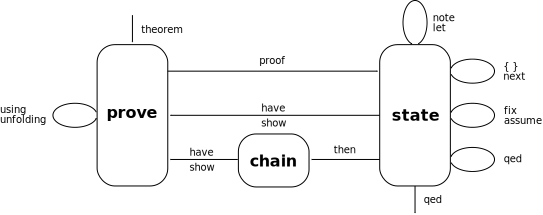
\includegraphics[width=0.8\textwidth]{Thy/document/isar-vm}
  \end{center}
  \caption{Isar/VM modes}\label{fig:isar-vm}
  \end{figure}

  For example, in \isa{{\isaliteral{22}{\isachardoublequote}}state{\isaliteral{22}{\isachardoublequote}}} mode Isar acts like a mathematical
  scratch-pad, accepting declarations like \hyperlink{command.fix}{\mbox{\isa{\isacommand{fix}}}}, \hyperlink{command.assume}{\mbox{\isa{\isacommand{assume}}}}, and claims like \hyperlink{command.have}{\mbox{\isa{\isacommand{have}}}}, \hyperlink{command.show}{\mbox{\isa{\isacommand{show}}}}.  A goal
  statement changes the mode to \isa{{\isaliteral{22}{\isachardoublequote}}prove{\isaliteral{22}{\isachardoublequote}}}, which means that we
  may now refine the problem via \hyperlink{command.unfolding}{\mbox{\isa{\isacommand{unfolding}}}} or \hyperlink{command.proof}{\mbox{\isa{\isacommand{proof}}}}.  Then we are again in \isa{{\isaliteral{22}{\isachardoublequote}}state{\isaliteral{22}{\isachardoublequote}}} mode of a proof body,
  which may issue \hyperlink{command.show}{\mbox{\isa{\isacommand{show}}}} statements to solve pending
  sub-goals.  A concluding \hyperlink{command.qed}{\mbox{\isa{\isacommand{qed}}}} will return to the original
  \isa{{\isaliteral{22}{\isachardoublequote}}state{\isaliteral{22}{\isachardoublequote}}} mode one level upwards.  The subsequent Isar/VM
  trace indicates block structure, linguistic mode, goal state, and
  inferences:%
\end{isamarkuptext}%
\isamarkuptrue%
%
\begingroup\footnotesize
%
\isadelimproof
%
\endisadelimproof
%
\isatagproof
%
\begin{minipage}[t]{0.18\textwidth}
\ \ \isacommand{have}\isamarkupfalse%
\ {\isaliteral{22}{\isachardoublequoteopen}}A\ {\isaliteral{5C3C6C6F6E6772696768746172726F773E}{\isasymlongrightarrow}}\ B{\isaliteral{22}{\isachardoublequoteclose}}\isanewline
\ \ \isacommand{proof}\isamarkupfalse%
\isanewline
\ \ \ \ \isacommand{assume}\isamarkupfalse%
\ A\isanewline
\ \ \ \ \isacommand{show}\isamarkupfalse%
\ B%
\endisatagproof
{\isafoldproof}%
%
\isadelimproof
%
\endisadelimproof
\isanewline
%
\isadelimnoproof
\ \ \ \ \ \ %
\endisadelimnoproof
%
\isatagnoproof
\isacommand{sorry}\isamarkupfalse%
%
\endisatagnoproof
{\isafoldnoproof}%
%
\isadelimnoproof
%
\endisadelimnoproof
\isanewline
%
\isadelimproof
\ \ %
\endisadelimproof
%
\isatagproof
\isacommand{qed}\isamarkupfalse%
%
\end{minipage}\quad
\begin{minipage}[t]{0.06\textwidth}
\isa{{\isaliteral{22}{\isachardoublequote}}begin{\isaliteral{22}{\isachardoublequote}}} \\
\\
\\
\isa{{\isaliteral{22}{\isachardoublequote}}begin{\isaliteral{22}{\isachardoublequote}}} \\
\isa{{\isaliteral{22}{\isachardoublequote}}end{\isaliteral{22}{\isachardoublequote}}} \\
\isa{{\isaliteral{22}{\isachardoublequote}}end{\isaliteral{22}{\isachardoublequote}}} \\
\end{minipage}
\begin{minipage}[t]{0.08\textwidth}
\isa{{\isaliteral{22}{\isachardoublequote}}prove{\isaliteral{22}{\isachardoublequote}}} \\
\isa{{\isaliteral{22}{\isachardoublequote}}state{\isaliteral{22}{\isachardoublequote}}} \\
\isa{{\isaliteral{22}{\isachardoublequote}}state{\isaliteral{22}{\isachardoublequote}}} \\
\isa{{\isaliteral{22}{\isachardoublequote}}prove{\isaliteral{22}{\isachardoublequote}}} \\
\isa{{\isaliteral{22}{\isachardoublequote}}state{\isaliteral{22}{\isachardoublequote}}} \\
\isa{{\isaliteral{22}{\isachardoublequote}}state{\isaliteral{22}{\isachardoublequote}}} \\
\end{minipage}\begin{minipage}[t]{0.35\textwidth}
\isa{{\isaliteral{22}{\isachardoublequote}}{\isaliteral{28}{\isacharparenleft}}A\ {\isaliteral{5C3C6C6F6E6772696768746172726F773E}{\isasymlongrightarrow}}\ B{\isaliteral{29}{\isacharparenright}}\ {\isaliteral{5C3C4C6F6E6772696768746172726F773E}{\isasymLongrightarrow}}\ {\isaliteral{23}{\isacharhash}}{\isaliteral{28}{\isacharparenleft}}A\ {\isaliteral{5C3C6C6F6E6772696768746172726F773E}{\isasymlongrightarrow}}\ B{\isaliteral{29}{\isacharparenright}}{\isaliteral{22}{\isachardoublequote}}} \\
\isa{{\isaliteral{22}{\isachardoublequote}}{\isaliteral{28}{\isacharparenleft}}A\ {\isaliteral{5C3C4C6F6E6772696768746172726F773E}{\isasymLongrightarrow}}\ B{\isaliteral{29}{\isacharparenright}}\ {\isaliteral{5C3C4C6F6E6772696768746172726F773E}{\isasymLongrightarrow}}\ {\isaliteral{23}{\isacharhash}}{\isaliteral{28}{\isacharparenleft}}A\ {\isaliteral{5C3C6C6F6E6772696768746172726F773E}{\isasymlongrightarrow}}\ B{\isaliteral{29}{\isacharparenright}}{\isaliteral{22}{\isachardoublequote}}} \\
\\
\\
\isa{{\isaliteral{22}{\isachardoublequote}}{\isaliteral{23}{\isacharhash}}{\isaliteral{28}{\isacharparenleft}}A\ {\isaliteral{5C3C6C6F6E6772696768746172726F773E}{\isasymlongrightarrow}}\ B{\isaliteral{29}{\isacharparenright}}{\isaliteral{22}{\isachardoublequote}}} \\
\isa{{\isaliteral{22}{\isachardoublequote}}A\ {\isaliteral{5C3C6C6F6E6772696768746172726F773E}{\isasymlongrightarrow}}\ B{\isaliteral{22}{\isachardoublequote}}} \\
\end{minipage}\begin{minipage}[t]{0.4\textwidth}
\isa{{\isaliteral{22}{\isachardoublequote}}{\isaliteral{28}{\isacharparenleft}}init{\isaliteral{29}{\isacharparenright}}{\isaliteral{22}{\isachardoublequote}}} \\
\isa{{\isaliteral{22}{\isachardoublequote}}{\isaliteral{28}{\isacharparenleft}}resolution\ impI{\isaliteral{29}{\isacharparenright}}{\isaliteral{22}{\isachardoublequote}}} \\
\\
\\
\isa{{\isaliteral{22}{\isachardoublequote}}{\isaliteral{28}{\isacharparenleft}}refinement\ {\isaliteral{23}{\isacharhash}}A\ {\isaliteral{5C3C4C6F6E6772696768746172726F773E}{\isasymLongrightarrow}}\ B{\isaliteral{29}{\isacharparenright}}{\isaliteral{22}{\isachardoublequote}}} \\
\isa{{\isaliteral{22}{\isachardoublequote}}{\isaliteral{28}{\isacharparenleft}}finish{\isaliteral{29}{\isacharparenright}}{\isaliteral{22}{\isachardoublequote}}} \\
\end{minipage}
%
\endisatagproof
{\isafoldproof}%
%
\isadelimproof
%
\endisadelimproof
%
\endgroup
%
\begin{isamarkuptext}%
\noindent Here the \hyperlink{inference.refinement}{\mbox{\isa{refinement}}} inference from
  \secref{sec:framework-resolution} mediates composition of Isar
  sub-proofs nicely.  Observe that this principle incorporates some
  degree of freedom in proof composition.  In particular, the proof
  body allows parameters and assumptions to be re-ordered, or commuted
  according to Hereditary Harrop Form.  Moreover, context elements
  that are not used in a sub-proof may be omitted altogether.  For
  example:%
\end{isamarkuptext}%
\isamarkuptrue%
%
\begin{minipage}{0.5\textwidth}
%
\isadelimproof
\ \ %
\endisadelimproof
%
\isatagproof
\isacommand{have}\isamarkupfalse%
\ {\isaliteral{22}{\isachardoublequoteopen}}{\isaliteral{5C3C416E643E}{\isasymAnd}}x\ y{\isaliteral{2E}{\isachardot}}\ A\ x\ {\isaliteral{5C3C4C6F6E6772696768746172726F773E}{\isasymLongrightarrow}}\ B\ y\ {\isaliteral{5C3C4C6F6E6772696768746172726F773E}{\isasymLongrightarrow}}\ C\ x\ y{\isaliteral{22}{\isachardoublequoteclose}}\isanewline
\ \ \isacommand{proof}\isamarkupfalse%
\ {\isaliteral{2D}{\isacharminus}}\isanewline
\ \ \ \ \isacommand{fix}\isamarkupfalse%
\ x\ \isakeyword{and}\ y\isanewline
\ \ \ \ \isacommand{assume}\isamarkupfalse%
\ {\isaliteral{22}{\isachardoublequoteopen}}A\ x{\isaliteral{22}{\isachardoublequoteclose}}\ \isakeyword{and}\ {\isaliteral{22}{\isachardoublequoteopen}}B\ y{\isaliteral{22}{\isachardoublequoteclose}}\isanewline
\ \ \ \ \isacommand{show}\isamarkupfalse%
\ {\isaliteral{22}{\isachardoublequoteopen}}C\ x\ y{\isaliteral{22}{\isachardoublequoteclose}}%
\endisatagproof
{\isafoldproof}%
%
\isadelimproof
%
\endisadelimproof
%
\isadelimnoproof
\ %
\endisadelimnoproof
%
\isatagnoproof
\isacommand{sorry}\isamarkupfalse%
%
\endisatagnoproof
{\isafoldnoproof}%
%
\isadelimnoproof
%
\endisadelimnoproof
\isanewline
%
\isadelimproof
\ \ %
\endisadelimproof
%
\isatagproof
\isacommand{qed}\isamarkupfalse%
%
\end{minipage}\begin{minipage}{0.5\textwidth}
\ \ \isacommand{have}\isamarkupfalse%
\ {\isaliteral{22}{\isachardoublequoteopen}}{\isaliteral{5C3C416E643E}{\isasymAnd}}x\ y{\isaliteral{2E}{\isachardot}}\ A\ x\ {\isaliteral{5C3C4C6F6E6772696768746172726F773E}{\isasymLongrightarrow}}\ B\ y\ {\isaliteral{5C3C4C6F6E6772696768746172726F773E}{\isasymLongrightarrow}}\ C\ x\ y{\isaliteral{22}{\isachardoublequoteclose}}\isanewline
\ \ \isacommand{proof}\isamarkupfalse%
\ {\isaliteral{2D}{\isacharminus}}\isanewline
\ \ \ \ \isacommand{fix}\isamarkupfalse%
\ x\ \isacommand{assume}\isamarkupfalse%
\ {\isaliteral{22}{\isachardoublequoteopen}}A\ x{\isaliteral{22}{\isachardoublequoteclose}}\isanewline
\ \ \ \ \isacommand{fix}\isamarkupfalse%
\ y\ \isacommand{assume}\isamarkupfalse%
\ {\isaliteral{22}{\isachardoublequoteopen}}B\ y{\isaliteral{22}{\isachardoublequoteclose}}\isanewline
\ \ \ \ \isacommand{show}\isamarkupfalse%
\ {\isaliteral{22}{\isachardoublequoteopen}}C\ x\ y{\isaliteral{22}{\isachardoublequoteclose}}%
\endisatagproof
{\isafoldproof}%
%
\isadelimproof
%
\endisadelimproof
%
\isadelimnoproof
\ %
\endisadelimnoproof
%
\isatagnoproof
\isacommand{sorry}\isamarkupfalse%
%
\endisatagnoproof
{\isafoldnoproof}%
%
\isadelimnoproof
%
\endisadelimnoproof
\isanewline
%
\isadelimproof
\ \ %
\endisadelimproof
%
\isatagproof
\isacommand{qed}\isamarkupfalse%
%
\end{minipage}\\[3ex]\begin{minipage}{0.5\textwidth}
\ \ \isacommand{have}\isamarkupfalse%
\ {\isaliteral{22}{\isachardoublequoteopen}}{\isaliteral{5C3C416E643E}{\isasymAnd}}x\ y{\isaliteral{2E}{\isachardot}}\ A\ x\ {\isaliteral{5C3C4C6F6E6772696768746172726F773E}{\isasymLongrightarrow}}\ B\ y\ {\isaliteral{5C3C4C6F6E6772696768746172726F773E}{\isasymLongrightarrow}}\ C\ x\ y{\isaliteral{22}{\isachardoublequoteclose}}\isanewline
\ \ \isacommand{proof}\isamarkupfalse%
\ {\isaliteral{2D}{\isacharminus}}\isanewline
\ \ \ \ \isacommand{fix}\isamarkupfalse%
\ y\ \isacommand{assume}\isamarkupfalse%
\ {\isaliteral{22}{\isachardoublequoteopen}}B\ y{\isaliteral{22}{\isachardoublequoteclose}}\isanewline
\ \ \ \ \isacommand{fix}\isamarkupfalse%
\ x\ \isacommand{assume}\isamarkupfalse%
\ {\isaliteral{22}{\isachardoublequoteopen}}A\ x{\isaliteral{22}{\isachardoublequoteclose}}\isanewline
\ \ \ \ \isacommand{show}\isamarkupfalse%
\ {\isaliteral{22}{\isachardoublequoteopen}}C\ x\ y{\isaliteral{22}{\isachardoublequoteclose}}\ \isacommand{sorry}\isamarkupfalse%
\isanewline
\ \ \isacommand{qed}\isamarkupfalse%
%
\end{minipage}\begin{minipage}{0.5\textwidth}
\ \ \isacommand{have}\isamarkupfalse%
\ {\isaliteral{22}{\isachardoublequoteopen}}{\isaliteral{5C3C416E643E}{\isasymAnd}}x\ y{\isaliteral{2E}{\isachardot}}\ A\ x\ {\isaliteral{5C3C4C6F6E6772696768746172726F773E}{\isasymLongrightarrow}}\ B\ y\ {\isaliteral{5C3C4C6F6E6772696768746172726F773E}{\isasymLongrightarrow}}\ C\ x\ y{\isaliteral{22}{\isachardoublequoteclose}}\isanewline
\ \ \isacommand{proof}\isamarkupfalse%
\ {\isaliteral{2D}{\isacharminus}}\isanewline
\ \ \ \ \isacommand{fix}\isamarkupfalse%
\ y\ \isacommand{assume}\isamarkupfalse%
\ {\isaliteral{22}{\isachardoublequoteopen}}B\ y{\isaliteral{22}{\isachardoublequoteclose}}\isanewline
\ \ \ \ \isacommand{fix}\isamarkupfalse%
\ x\isanewline
\ \ \ \ \isacommand{show}\isamarkupfalse%
\ {\isaliteral{22}{\isachardoublequoteopen}}C\ x\ y{\isaliteral{22}{\isachardoublequoteclose}}\ \isacommand{sorry}\isamarkupfalse%
\isanewline
\ \ \isacommand{qed}\isamarkupfalse%
%
\endisatagproof
{\isafoldproof}%
%
\isadelimproof
%
\endisadelimproof
%
\end{minipage}
%
\begin{isamarkuptext}%
\medskip\noindent Such ``peephole optimizations'' of Isar texts are
  practically important to improve readability, by rearranging
  contexts elements according to the natural flow of reasoning in the
  body, while still observing the overall scoping rules.

  \medskip This illustrates the basic idea of structured proof
  processing in Isar.  The main mechanisms are based on natural
  deduction rule composition within the Pure framework.  In
  particular, there are no direct operations on goal states within the
  proof body.  Moreover, there is no hidden automated reasoning
  involved, just plain unification.%
\end{isamarkuptext}%
\isamarkuptrue%
%
\isamarkupsubsection{Calculational reasoning \label{sec:framework-calc}%
}
\isamarkuptrue%
%
\begin{isamarkuptext}%
The existing Isar infrastructure is sufficiently flexible to support
  calculational reasoning (chains of transitivity steps) as derived
  concept.  The generic proof elements introduced below depend on
  rules declared as \hyperlink{attribute.trans}{\mbox{\isa{trans}}} in the context.  It is left to
  the object-logic to provide a suitable rule collection for mixed
  relations of \isa{{\isaliteral{22}{\isachardoublequote}}{\isaliteral{3D}{\isacharequal}}{\isaliteral{22}{\isachardoublequote}}}, \isa{{\isaliteral{22}{\isachardoublequote}}{\isaliteral{3C}{\isacharless}}{\isaliteral{22}{\isachardoublequote}}}, \isa{{\isaliteral{22}{\isachardoublequote}}{\isaliteral{5C3C6C653E}{\isasymle}}{\isaliteral{22}{\isachardoublequote}}}, \isa{{\isaliteral{22}{\isachardoublequote}}{\isaliteral{5C3C7375627365743E}{\isasymsubset}}{\isaliteral{22}{\isachardoublequote}}},
  \isa{{\isaliteral{22}{\isachardoublequote}}{\isaliteral{5C3C73756273657465713E}{\isasymsubseteq}}{\isaliteral{22}{\isachardoublequote}}} etc.  Due to the flexibility of rule composition
  (\secref{sec:framework-resolution}), substitution of equals by
  equals is covered as well, even substitution of inequalities
  involving monotonicity conditions; see also \cite[\S6]{Wenzel-PhD}
  and \cite{Bauer-Wenzel:2001}.

  The generic calculational mechanism is based on the observation that
  rules such as \isa{{\isaliteral{22}{\isachardoublequote}}trans{\isaliteral{3A}{\isacharcolon}}{\isaliteral{22}{\isachardoublequote}}}~\isa{{\isaliteral{22}{\isachardoublequote}}x\ {\isaliteral{3D}{\isacharequal}}\ y\ {\isaliteral{5C3C4C6F6E6772696768746172726F773E}{\isasymLongrightarrow}}\ y\ {\isaliteral{3D}{\isacharequal}}\ z\ {\isaliteral{5C3C4C6F6E6772696768746172726F773E}{\isasymLongrightarrow}}\ x\ {\isaliteral{3D}{\isacharequal}}\ z{\isaliteral{22}{\isachardoublequote}}}
  proceed from the premises towards the conclusion in a deterministic
  fashion.  Thus we may reason in forward mode, feeding intermediate
  results into rules selected from the context.  The course of
  reasoning is organized by maintaining a secondary fact called
  ``\hyperlink{fact.calculation}{\mbox{\isa{calculation}}}'', apart from the primary ``\hyperlink{fact.this}{\mbox{\isa{this}}}''
  already provided by the Isar primitives.  In the definitions below,
  \hyperlink{attribute.OF}{\mbox{\isa{OF}}} refers to \hyperlink{inference.resolution}{\mbox{\isa{resolution}}}
  (\secref{sec:framework-resolution}) with multiple rule arguments,
  and \isa{{\isaliteral{22}{\isachardoublequote}}trans{\isaliteral{22}{\isachardoublequote}}} represents to a suitable rule from the context:

  \begin{matharray}{rcl}
    \hyperlink{command.also}{\mbox{\isa{\isacommand{also}}}}\isa{{\isaliteral{22}{\isachardoublequote}}\isaliteral{5C3C5E7375623E}{}\isactrlsub {\isadigit{0}}{\isaliteral{22}{\isachardoublequote}}} & \equiv & \hyperlink{command.note}{\mbox{\isa{\isacommand{note}}}}~\isa{{\isaliteral{22}{\isachardoublequote}}calculation\ {\isaliteral{3D}{\isacharequal}}\ this{\isaliteral{22}{\isachardoublequote}}} \\
    \hyperlink{command.also}{\mbox{\isa{\isacommand{also}}}}\isa{{\isaliteral{22}{\isachardoublequote}}\isaliteral{5C3C5E7375623E}{}\isactrlsub n\isaliteral{5C3C5E7375623E}{}\isactrlsub {\isaliteral{2B}{\isacharplus}}\isaliteral{5C3C5E7375623E}{}\isactrlsub {\isadigit{1}}{\isaliteral{22}{\isachardoublequote}}} & \equiv & \hyperlink{command.note}{\mbox{\isa{\isacommand{note}}}}~\isa{{\isaliteral{22}{\isachardoublequote}}calculation\ {\isaliteral{3D}{\isacharequal}}\ trans\ {\isaliteral{5B}{\isacharbrackleft}}OF\ calculation\ this{\isaliteral{5D}{\isacharbrackright}}{\isaliteral{22}{\isachardoublequote}}} \\[0.5ex]
    \hyperlink{command.finally}{\mbox{\isa{\isacommand{finally}}}} & \equiv & \hyperlink{command.also}{\mbox{\isa{\isacommand{also}}}}~\hyperlink{command.from}{\mbox{\isa{\isacommand{from}}}}~\isa{calculation} \\
  \end{matharray}

  \noindent The start of a calculation is determined implicitly in the
  text: here \hyperlink{command.also}{\mbox{\isa{\isacommand{also}}}} sets \hyperlink{fact.calculation}{\mbox{\isa{calculation}}} to the current
  result; any subsequent occurrence will update \hyperlink{fact.calculation}{\mbox{\isa{calculation}}} by
  combination with the next result and a transitivity rule.  The
  calculational sequence is concluded via \hyperlink{command.finally}{\mbox{\isa{\isacommand{finally}}}}, where
  the final result is exposed for use in a concluding claim.

  Here is a canonical proof pattern, using \hyperlink{command.have}{\mbox{\isa{\isacommand{have}}}} to
  establish the intermediate results:%
\end{isamarkuptext}%
\isamarkuptrue%
%
\isadelimproof
\ \ %
\endisadelimproof
%
\isatagproof
\isacommand{have}\isamarkupfalse%
\ {\isaliteral{22}{\isachardoublequoteopen}}a\ {\isaliteral{3D}{\isacharequal}}\ b{\isaliteral{22}{\isachardoublequoteclose}}\ \isacommand{sorry}\isamarkupfalse%
\isanewline
\ \ \isacommand{also}\isamarkupfalse%
\ \isacommand{have}\isamarkupfalse%
\ {\isaliteral{22}{\isachardoublequoteopen}}{\isaliteral{5C3C646F74733E}{\isasymdots}}\ {\isaliteral{3D}{\isacharequal}}\ c{\isaliteral{22}{\isachardoublequoteclose}}\ \isacommand{sorry}\isamarkupfalse%
\isanewline
\ \ \isacommand{also}\isamarkupfalse%
\ \isacommand{have}\isamarkupfalse%
\ {\isaliteral{22}{\isachardoublequoteopen}}{\isaliteral{5C3C646F74733E}{\isasymdots}}\ {\isaliteral{3D}{\isacharequal}}\ d{\isaliteral{22}{\isachardoublequoteclose}}\ \isacommand{sorry}\isamarkupfalse%
\isanewline
\ \ \isacommand{finally}\isamarkupfalse%
\ \isacommand{have}\isamarkupfalse%
\ {\isaliteral{22}{\isachardoublequoteopen}}a\ {\isaliteral{3D}{\isacharequal}}\ d{\isaliteral{22}{\isachardoublequoteclose}}\ \isacommand{{\isaliteral{2E}{\isachardot}}}\isamarkupfalse%
%
\endisatagproof
{\isafoldproof}%
%
\isadelimproof
%
\endisadelimproof
%
\begin{isamarkuptext}%
\noindent The term ``\isa{{\isaliteral{22}{\isachardoublequote}}{\isaliteral{5C3C646F74733E}{\isasymdots}}{\isaliteral{22}{\isachardoublequote}}}'' above is a special abbreviation
  provided by the Isabelle/Isar syntax layer: it statically refers to
  the right-hand side argument of the previous statement given in the
  text.  Thus it happens to coincide with relevant sub-expressions in
  the calculational chain, but the exact correspondence is dependent
  on the transitivity rules being involved.

  \medskip Symmetry rules such as \isa{{\isaliteral{22}{\isachardoublequote}}x\ {\isaliteral{3D}{\isacharequal}}\ y\ {\isaliteral{5C3C4C6F6E6772696768746172726F773E}{\isasymLongrightarrow}}\ y\ {\isaliteral{3D}{\isacharequal}}\ x{\isaliteral{22}{\isachardoublequote}}} are like
  transitivities with only one premise.  Isar maintains a separate
  rule collection declared via the \hyperlink{attribute.sym}{\mbox{\isa{sym}}} attribute, to be
  used in fact expressions ``\isa{{\isaliteral{22}{\isachardoublequote}}a\ {\isaliteral{5B}{\isacharbrackleft}}symmetric{\isaliteral{5D}{\isacharbrackright}}{\isaliteral{22}{\isachardoublequote}}}'', or single-step
  proofs ``\hyperlink{command.assume}{\mbox{\isa{\isacommand{assume}}}}~\isa{{\isaliteral{22}{\isachardoublequote}}x\ {\isaliteral{3D}{\isacharequal}}\ y{\isaliteral{22}{\isachardoublequote}}}~\hyperlink{command.then}{\mbox{\isa{\isacommand{then}}}}~\hyperlink{command.have}{\mbox{\isa{\isacommand{have}}}}~\isa{{\isaliteral{22}{\isachardoublequote}}y\ {\isaliteral{3D}{\isacharequal}}\ x{\isaliteral{22}{\isachardoublequote}}}~\hyperlink{command.ddot}{\mbox{\isa{\isacommand{{\isaliteral{2E}{\isachardot}}{\isaliteral{2E}{\isachardot}}}}}}''.%
\end{isamarkuptext}%
\isamarkuptrue%
%
\isadelimtheory
%
\endisadelimtheory
%
\isatagtheory
\isacommand{end}\isamarkupfalse%
%
\endisatagtheory
{\isafoldtheory}%
%
\isadelimtheory
%
\endisadelimtheory
\end{isabellebody}%
%%% Local Variables:
%%% mode: latex
%%% TeX-master: "root"
%%% End:
